\newpage
\section{PHƯƠNG TRÌNH LƯỢNG GIÁC CƠ BẢN}
\subsection{LÝ THUYẾT CẦN NHỚ}
\subsubsection{Phương trình tương đương}
\indam{Định nghĩa:}
\begin{boxdn}
\begin{itemize}
\item Hai phương trình được gọi là \textbf{tương đương} nếu chúng có cùng tập nghiệm. 
\item Để chỉ sự tương đương của các phương trình, người ta dùng kí hiệu \lq\lq $\Leftrightarrow $\rq\rq.
\end{itemize}
\end{boxdn}

\subsubsection{Phương trình sin x = m}
\begin{boxdn}
Xét phương trình $\sin x = m$
\begin{itemize}
\item Nếu $|m| > 1$ thì phương trình vô nghiệm.
\item Nếu $|m| \le 1$ thì phương trình có nghiệm $\hoac{&x=\alpha + k2 \pi\\&x=\pi-\alpha + k2 \pi}, k\in \mathbb{Z}$, với $\alpha \in \left[ - \dfrac{\pi}{2}; \dfrac{\pi}{2}\right]$ sao cho $\sin \alpha =m$.
\end{itemize}
\end{boxdn}

\begin{khung4}{Chú ý}
\begin{enumerate}
\item Một số trường hợp đặc biệt:
\begin{itemize}
\item $\sin x = 1 \Leftrightarrow x= \dfrac{\pi}{2} + k2\pi$, $k\in \mathbb{Z}$;
\item $\sin x =- 1 \Leftrightarrow x= -\dfrac{\pi}{2} + k2\pi$, $k\in \mathbb{Z}$;
\item $\sin x =0 \Leftrightarrow x= k\pi$, $k\in \mathbb{Z}$.
\end{itemize}
\item $\sin x = \sin a^\circ \Leftrightarrow \hoac{&x = a^\circ + k 360^\circ\\&x = 180^\circ - a^\circ + k 360^\circ }, k\in \mathbb{Z}$.
\item $\sin u = \sin v \Leftrightarrow \hoac{&u = v + k2\pi\\&u=\pi -v + k2\pi},k\in \mathbb{Z}$.
\end{enumerate}
\end{khung4}

\subsubsection{Phương trình cos x = m}
\begin{boxdn}
Xét phương trình $\cos x = m$
\begin{itemize}
\item Nếu $|m| > 1$ thì phương trình vô nghiệm.
\item Nếu $|m| \le 1$ thì phương trình có nghiệm $\hoac{&x=\alpha + k2 \pi\\&x=-\alpha + k2 \pi}, k\in \mathbb{Z}$, với $\alpha \in [ 0; \pi]$ sao cho $\cos \alpha =m$.
\end{itemize}
\end{boxdn}

\begin{khung4}{Chú ý}
\begin{enumerate}
\item Một số trường hợp đặc biệt:
\begin{itemize}
\item $\cos x = 1 \Leftrightarrow x=  k2\pi$, $k\in \mathbb{Z}$;
\item $\cos x =- 1 \Leftrightarrow x= \pi + k2\pi$, $k\in \mathbb{Z}$;
\item $\cos x =0 \Leftrightarrow x= \dfrac{\pi}{2}+ k\pi$, $k\in \mathbb{Z}$.
\end{itemize}
\item $\cos x = \cos a^\circ \Leftrightarrow \hoac{&x = a^\circ + k 360^\circ\\&x =  - a^\circ + k 360^\circ },k\in \mathbb{Z}$.
\item $\cos u = \cos v \Leftrightarrow \hoac{&u = v + k2\pi\\&u= -v + k2\pi},k\in \mathbb{Z}$.
\end{enumerate}
\end{khung4}

\subsubsection{Phương trình tan x = m }
\begin{boxdn}
Với mọi số thực $m$, phương trình $\tan x = m$ có nghiệm $x = \alpha +k\pi$, $k \in \mathbb{Z}$, với $\alpha\in \left( -\dfrac{\pi}{2}; \dfrac{\pi}{2} \right)$ sao cho $\tan x = m$.
\end{boxdn}


\begin{khung4}{Chú ý}
$\tan x = \tan a^\circ \Leftrightarrow x = a^\circ + k180^\circ$, $k \in \mathbb{Z}$.
\end{khung4}

\subsubsection{Phương trình cot x = m}
\begin{boxdn}
Với mọi số thực $m$, phương trình $\cot x = m$ có nghiệm $x = \alpha + k\pi$, $k \in \mathbb{Z}$ với $\alpha\in \left( 0; \pi \right)$ sao cho $\cot x = m$.
\end{boxdn}

\begin{khung4}{Chú ý}
$\cot x = \cot a^\circ \Leftrightarrow x = a^\circ + k180^\circ$, $k \in \mathbb{Z}$.
\end{khung4}
%-------------------------------------------------------------------------------------------------------------
\subsection{PHÂN LOẠI VÀ PHƯƠNG PHÁP GIẢI TOÁN}
\begin{dang}{Câu hỏi lý thuyết, khái niệm phương trình tương đương}
\end{dang}

\begin{vd}%[1D1B5-1]
Các phép biến đổi sau có phải là phép biến đổi tương đương không? Vì sao?
\begin{enumerate}
\item  $(x-1) \sin x=(x-1) \cos x \Leftrightarrow \sin x=\cos x$;
\item  $\dfrac{2 x^2}{x^2+1}=1 \Leftrightarrow 2 x^2=x^2+1$. 
\end{enumerate}
\loigiai{
\begin{enumerate}
\item  Phép biến đổi này không là phép biến đổi tương đương vì $x=1$ là một nghiệm của phương trình $(x-1) \sin x=(x-1) \cos x$ nhưng lại không là nghiệm của phương trình $\sin x=\cos x$. \\
Lưu ý rằng khi nhân hoặc chia hai vế của phương trình với cùng một biểu thức có thể nhận giá trị bằng 0 thì ta chưa thể kết luận phương trình thu được tương đương với phương trình ban đầu.
\item  Phép biến đổi này là phép biến đổi tương đương vì ta đã nhân hai vế của phương trình $\dfrac{2 x^2}{x^2+1}=1$ với biểu thức luôn có giá trị dương với mọi số thực $x$ là $x^2+1$.
\end{enumerate}
}
\end{vd}

\begin{dang}{Điều kiện để phương trình có nghiệm}
\end{dang}

\begin{vd}
Tìm điều kiện của $m$ để phương trình $\sin \dfrac{x}{2}=m$ có nghiệm.
\loigiai{
Ta có $-1\le \sin \dfrac{x}{2}\le 1$ $\Rightarrow $ $-1\le m\le 1$. Vậy $m\in \left[-1;1\right]$.}
\end{vd}

\begin{vd}
Tìm điều kiện của $m$ để phương trình $\cos x =m$ có nghiệm trên khoảng $\left(-\dfrac{\pi}{2};\dfrac{\pi}{2}\right)$.
\loigiai{
Đồ thị của hàm số $y=\cos x$ trên khoảng $\left(-\dfrac{\pi}{2};\dfrac{\pi}{2} \right)$ như hình vẽ.
\begin{center}
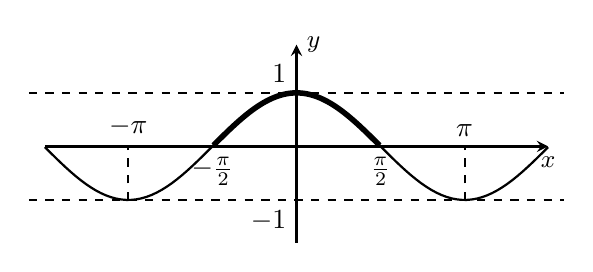
\begin{tikzpicture}[thick,>=stealth,x=1cm,y=1cm,scale=0.68] 
\draw[->] (-4.7,0) -- (4.7,0) node[below] {\small $x$};
\draw[->] (0,-1.8) -- (0,1.9) node[right] {\small $y$};
\draw[line width=2pt,samples=100,domain=-1.55:1.55] plot(\x,{cos((\x)*180/pi)});
\draw[thick,samples=100,domain=-4.7:4.7] plot(\x,{cos((\x)*180/pi)});
\draw[dashed] (-3.14,-1)--(-3.14,0) node[above] {$-\pi$};
\draw[dashed] (3.14,-1)--(3.14,0) node[above] {$\pi$};
\draw (-1.57,0) node[below] {$-\frac{\pi}{2}$};
\draw (1.57,0) node[below] {$\frac{\pi}{2}$};
\draw[dashed] (-5,1)--(0,1) node[above left]{$1$}--(5,1);
\draw[dashed] (-5,-1)--(0,-1)node[below left]{$-1$}--(5,-1);
\end{tikzpicture}
\end{center}
Phương trình $\cos x =m$ có nghiệm trên khoảng $\left(-\dfrac{\pi}{2};\dfrac{\pi}{2}\right)$ khi $0<m<1$.
}
\end{vd}

\begin{dang}{Phương trình cơ bản theo đơn vị radian}
\end{dang} 
\begin{vd}%[1D1B5-3] 
Giải phương trình 
\begin{listEX}[2]
\item $\sin \left(2x-\dfrac{\pi}{3}\right)= - \dfrac{\sqrt{3}}{2}$;
\item $\cos \left(\dfrac{x}{2}+\dfrac{\pi}{4}\right)= \dfrac{\sqrt{3}}{2}$;
\item $\tan \left(3x+\dfrac{\pi}{4}\right)= \dfrac{\sqrt{3}}{3}$;
\item $\sqrt{3}\cot \left(2x-\dfrac{\pi}{6}\right)= - 1$.
\end{listEX}
\loigiai{
\begin{enumerate}
\item $\sin \left(2x-\dfrac{\pi}{3}\right)=-\dfrac{\sqrt{3}}{2}\Leftrightarrow \sin \left(2x-\dfrac{\pi}{3}\right)=\sin\left(-\dfrac{\pi}{3}\right) \Leftrightarrow \hoac{&2x - \dfrac {\pi}{3} = - \dfrac {\pi}{3} + k2\pi \\& 2x - \dfrac {\pi}{3} = \pi - \left( - \dfrac{\pi}{3}\right) + k2\pi}\Leftrightarrow \hoac{&x=k \pi \\ &x=\dfrac{5 \pi}{6}+k\pi} (k \in \mathbb{Z}).$
\item  $\cos \left(\dfrac{x}{2}+\dfrac{\pi}{4}\right)=\dfrac{\sqrt{3}}{2} \Leftrightarrow \cos \left(\dfrac{x}{2}+\dfrac{\pi}{4}\right)=\cos \dfrac{\pi}{6} \Leftrightarrow \hoac{&\dfrac {x}{2} + \dfrac {\pi}{4} = \dfrac {\pi}{6} + k2 \pi \\&\dfrac {x}{2} + \dfrac {\pi}{4} = - \dfrac {\pi}{6} + k2\pi }
\Leftrightarrow \hoac{&x=-\dfrac{\pi}{6}+k 4 \pi \\&x=-\dfrac{5 \pi}{6}+k 4 \pi} (k \in \mathbb{Z}).$
\item $\tan \left(3 x+\dfrac{\pi}{4}\right)=\dfrac{\sqrt{3}}{3} \Leftrightarrow \tan \left(3 x+\dfrac{\pi}{4}\right)=\tan \dfrac{\pi}{6} \Leftrightarrow 3 x+\dfrac{\pi}{4}=\dfrac{\pi}{6}+k \pi \Leftrightarrow x=-\dfrac{\pi}{36}+k \dfrac{\pi}{3}\ (k \in \mathbb{Z}).$
\item $\sqrt{3} \cot \left(2 x-\dfrac{\pi}{6}\right)=-1 \Leftrightarrow \cot \left(2 x-\dfrac{\pi}{6}\right)=-\dfrac{1}{\sqrt{3}}\Leftrightarrow \cot \left(2 x-\dfrac{\pi}{6}\right)=\cot \dfrac{2 \pi}{3}\Leftrightarrow 2 x-\dfrac{\pi}{6}=\dfrac{2 \pi}{3}+k \pi \Leftrightarrow x=\dfrac{5 \pi}{12}+k \dfrac{\pi}{2}\ (k \in \mathbb{Z}).$
\end{enumerate}
}
\end{vd}

\begin{vd}%[1D1B5-3]
Tìm nghiệm của phương trình
\begin{listEX}[2]
\item $\sin \left(2x+\dfrac{2\pi}{5}\right)=0$ với $x\in \left(\dfrac{\pi}{2};\dfrac{3\pi}{2}\right)$;
\item $\tan \left(\dfrac{x}{2}+\dfrac{\pi}{6}\right)=-1$ với $x\in \left(-\dfrac{\pi}{2};\dfrac{\pi}{2}\right)$.
\end{listEX}
\loigiai{
\begin{enumerate}
\item $\sin \left(2 x+\dfrac{2 \pi}{5}\right)=0 \Leftrightarrow 2x+\dfrac{2 \pi}{5}=k \pi \Leftrightarrow x=-\dfrac{\pi}{5}+k \dfrac{\pi}{2}$.\\
Do $x \in\left(\dfrac{\pi}{2}; \dfrac{3 \pi}{2}\right)$ nên $\dfrac{\pi}{2}<-\dfrac{\pi}{5}+k \dfrac{\pi}{2}<\dfrac{3 \pi}{2} \Leftrightarrow \dfrac{7}{5}<k<\dfrac{17}{5}$.\\
Mà $k \in \mathbb{Z}$ nên $k \in\{2; 3\}$. Vậy $x \in\left\{\dfrac{4 \pi}{5} ; \dfrac{13 \pi}{10}\right\}$.
\item $\tan \left(\dfrac{x}{2}+\dfrac{\pi}{6}\right)=-1 \Leftrightarrow \dfrac{x}{2}+\dfrac{\pi}{6}=-\dfrac{\pi}{4}+k \pi \Leftrightarrow x=-\dfrac{5 \pi}{6}+k 2\pi$.\\
Do $x \in\left(-\dfrac{\pi}{2}; \dfrac{\pi}{2}\right)$ nên $-\dfrac{\pi}{2}<-\dfrac{5 \pi}{6}+k 2 \pi<\dfrac{\pi}{2} \Leftrightarrow \dfrac{1}{6}<k<\dfrac{2}{3}$.\\
Mà $k \in \mathbb{Z}$ nên không có giá trị nào của $k$ thoả mãn. \\
Vậy phương trình không có nghiệm trên khoảng $\left(-\dfrac{\pi}{2} ; \dfrac{\pi}{2}\right)$.
\end{enumerate}
}
\end{vd}

\begin{dang}{Phương trình cơ bản theo đơn vị độ}
\end{dang}

\begin{vd}%[1D1B5-4]
Giải các phương trình lượng giác sau:
\begin{enumEX}{2}
\item $\sin 2x=\sin 42^\circ$;
\item $2\cos (-2x + 17^\circ) = 4$;
\item $\tan x=\tan 25^\circ$;
\item $\cot x=\cot (-32^\circ)$.
\end{enumEX}
\loigiai{
\begin{enumerate}
\item 
$\sin 2x=\sin 42^\circ \Leftrightarrow\hoac{&2x=42^\circ+k360^\circ\\&2x=180^\circ-42^\circ+k360^\circ}\Leftrightarrow\hoac{&x=21^\circ+k180^\circ\\&x=69^\circ+k180^\circ},\, (k\in\mathbb{Z})$.
\item 
$2\cos (-2x + 17^\circ) = 4 \Leftrightarrow \cos (-2x + 17^\circ) = 2$.
Vậy phương trình vô nghiệm.
\item 
$\tan x=\tan 25^\circ\Leftrightarrow x=25^\circ+k180^\circ,\, (k\in\mathbb{Z})$.
\item 
$\cot x=\cot (-32^\circ)\Leftrightarrow x=-32^\circ+k180^\circ,\, (k\in\mathbb{Z})$.
\end{enumerate}
}
\end{vd}

\begin{dang}{Phương trình đưa về dạng cơ bản}
\end{dang}

\begin{vd}%[1D1B5-3]
Giải các phương trình lượng giác sau:
\begin{enumEX}{2}
\item $\cos 2x=\cos (3x+10^\circ)$;
\item $\tan (x - 30^\circ ) - \cot 50^\circ = 0$;
\item $\cos x+\sin x=0$;
\item $\sin x-\sqrt{3}\cos x=0$;
\item $\cos (2x  +10^\circ) = \sin (50^\circ - x)$;
\item $\tan (x - 30^\circ ) - \cot 50^\circ = 0$;
\item $\cos \left( 3x - \dfrac{7\pi}{12} \right) = \cos \left( - x + \dfrac{\pi}{4} \right)$;
\item $\cot \left( \dfrac{x}{3} + \dfrac{2\pi}{5} \right) =\cot \dfrac{\pi}{5}$.
\item $\cos \left( x + \dfrac{\pi}{4} \right) + \cos \left( \dfrac{\pi}{4} - x \right) = 0$;
\item $\sin \left(3x-\dfrac{\pi}{4}\right)=\sin\left(x+\dfrac{\pi}{6}\right)$;
\item $\cos\left(2x-\dfrac{\pi}{3}\right)=\sin\left(\dfrac{\pi}{4}-x\right)$;
\item $\cos\left(2x+\dfrac{\pi}{5}\right)+\cos\left(3x-\dfrac{\pi}{6}\right)=0$.
\end{enumEX}
\loigiai{
\begin{enumerate}
\item 
$\cos 2x=\cos (3x+10^\circ) \Leftrightarrow\hoac{&2x=3x+10^\circ+k360^\circ\\&2x=-3x-10^\circ+k360^\circ}\Leftrightarrow\hoac{&-x=10^\circ+k360^\circ\\&5x=-10^\circ+k360^\circ}\Leftrightarrow\hoac{&x=-10^\circ-k360^\circ\\&x=-2^\circ+k72^\circ},\, (k\in\mathbb{Z})$.
\item 
$\tan (x - 30^\circ ) - \cot 50^\circ = 0 \Leftrightarrow \tan (x - 30^\circ ) = \tan 40^\circ \Leftrightarrow x - 30^\circ =  40^\circ + k 180^\circ \Leftrightarrow x = 70^\circ + k 180^\circ, (k\in\mathbb{Z})$.
\item $\cos x+\sin x=0\Leftrightarrow \sin x=-\cos x\Leftrightarrow \tan x=-1\Leftrightarrow x=-\dfrac{\pi}{4}+k\pi,\, (k\in\mathbb{Z})$.
\item $\sin x-\sqrt{3}\cos x=0\Leftrightarrow \sin x=\sqrt{3}\cos x\Leftrightarrow \tan x=\sqrt{3}\Leftrightarrow x=\dfrac{\pi}{3}+k\pi,\, (k\in\mathbb{Z})$.
\item $\cos (2x  +10^\circ) = \sin (50^\circ - x) \Leftrightarrow \cos (2x  +10^\circ) = \cos (x + 40^\circ) \Leftrightarrow \hoac{& x = 30^\circ + k360^\circ \\ & x = -\dfrac{1}{3}\cdot 50^\circ + k 210^\circ}, (k\in\mathbb{Z})$.
\item $\tan (x - 30^\circ ) - \cot 50^\circ = 0 \Leftrightarrow \tan (x - 30^\circ ) = \tan 40^\circ \Leftrightarrow x - 30^\circ =  40^\circ + k 180^\circ \Leftrightarrow x = 70^\circ + k 180^\circ, (k\in\mathbb{Z})$.
\item $\cos \left( 3x - \dfrac{7\pi}{12} \right) = \cos \left( - x + \dfrac{\pi}{4} \right)  \Leftrightarrow \hoac{& 3x - \dfrac{7\pi}{12} = - x + \dfrac{\pi}{4} + k2\pi\\ & 3x - \dfrac{7\pi}{12} = x - \dfrac{\pi}{4} + k2\pi} \Leftrightarrow \hoac{& x = \dfrac{5\pi}{24} + k \dfrac{\pi}{2}\\ & x = \dfrac{\pi}{6} + k\pi}, (k\in\mathbb{Z})$.
\item $\cot \left( \dfrac{x}{3} + \dfrac{2\pi}{5} \right) =\cot \dfrac{\pi}{5} \Leftrightarrow \dfrac{x}{3} + \dfrac{2\pi}{5} = \dfrac{\pi}{5} + k\pi \Leftrightarrow x = - \dfrac{3\pi}{5} + k3\pi, (k\in\mathbb{Z})$.
\item $\cos \left( x + \dfrac{\pi}{4} \right) + \cos \left( \dfrac{\pi}{4} - x \right) = 0 \Leftrightarrow \cos \left( x + \dfrac{\pi}{4} \right) =  \cos \left( \dfrac{3\pi}{4} + x \right)\Leftrightarrow \hoac{& x + \dfrac{\pi}{4} = \dfrac{3\pi}{4} + x + k2\pi \text{ (vô nghiệm)} \\ & x + \dfrac{\pi}{4} = - \dfrac{3\pi}{4} - x + k2\pi} \Leftrightarrow x = - \dfrac{\pi}{2}  + k\pi$.
\item $\sin \left(3x-\dfrac{\pi}{4}\right)=\sin\left(x+\dfrac{\pi}{6}\right)\Leftrightarrow\hoac{&3x-\dfrac{\pi}{4}=x+\dfrac{\pi}{6}+k2\pi\\&3x-\dfrac{\pi}{4}=\pi-x-\dfrac{\pi}{6}+k2\pi} \Leftrightarrow\hoac{&2x=\dfrac{5\pi}{12}+k2\pi\\&4x=\dfrac{\pi}{12}+k2\pi} \Leftrightarrow\hoac{&x=\dfrac{5\pi}{24}+k\pi\\&x=\dfrac{\pi}{48}+\dfrac{k\pi}{2}}\, (k\in\mathbb{Z}).$
\item $\cos\left(2x-\dfrac{\pi}{3}\right)=\sin\left(\dfrac{\pi}{4}-x\right)\Leftrightarrow\cos\left(2x-\dfrac{\pi}{3}\right)=\cos\left(\dfrac{\pi}{2}-\dfrac{\pi}{4}+x\right)
\Leftrightarrow\hoac{&2x-\dfrac{\pi}{3}=\dfrac{\pi}{2}-\dfrac{\pi}{4}+x+k2\pi\\&2x-\dfrac{\pi}{3}=-\dfrac{\pi}{2}+\dfrac{\pi}{4}-x+k2\pi}
\Leftrightarrow\hoac{&x=\dfrac{7\pi}{12}+k2\pi\\&x=\dfrac{\pi}{36}+k\dfrac{2\pi}{3}}\, (k\in\mathbb{Z}).$
\item $\cos\left(2x+\dfrac{\pi}{5}\right)+\cos\left(3x-\dfrac{\pi}{6}\right)=0
\Leftrightarrow\cos\left(2x+\dfrac{\pi}{5}\right)=\cos\left(3x+\dfrac{5\pi}{6}\right)
\Leftrightarrow\hoac{&2x+\dfrac{\pi}{5}=3x+\dfrac{5\pi}{6}+k2\pi\\&2x+\dfrac{\pi}{5}=-3x-\dfrac{5\pi}{6}+k2\pi}
\Leftrightarrow\hoac{&x=-\dfrac{19\pi}{30}-k2\pi\\&x=-\dfrac{31\pi}{150}+k\dfrac{2\pi}{5}} .$
\end{enumerate}
}
\end{vd}

\begin{dang}{Vận dụng phương trình lượng giác để giải các bài toán thực tế}
\end{dang}

\begin{vd}%[1D1K5-6]
\immini{Hội Lim (tỉnh Bắc Ninh) được tổ chức vào mùa xuân thường có trò chơi đánh đu. 
Khi người chơi đu nhún đều, cây đu sẽ đưa người chơi đu dao động quanh vị trí cân bằng (hình bên). Nghiên cứu trò chơi này, người ta thấy khoảng cách $h$ (m) từ vị trí người chơi đu đến vị trí cân bằng được biểu diễn qua thời gian $t\,(s)$ (với $t\geq 0$) vởi hệ thức $h=|d|$ với $d=3\cos \left[\dfrac{\pi}{3}(2t-1)\right]$, trong đó ta quy ước $d>0$ khi vị trí cân bằng ở phía sau lưng người chơi đu và $d<0$ trong trường hợp ngược lại. Vào thời điểm $t$ nào thì khoảng cách $h$ là $3$ m; $0$ m?
}{
\begin{tikzpicture}[>=stealth,scale=0.7, line join = round, line cap = round]
\path (0,0.3) coordinate (A) 
(0,-5.5) coordinate (B)
(-110:5) coordinate (C)
($(A)!(C)!(B)$) coordinate (H)
;
\draw[fill] (0,0) circle (1.5pt) (-50:5)circle (1.5pt) (-130:5) circle (1.5pt) (-110:5) circle (1.5pt);
\draw[dashed,midway] (A)--(B) node[midway,rotate=90,below]{Vị trí cân bằng};
\draw[dashed] (-50:5)--(0,0)--(-130:5);
\draw (0,0)--(-110:5);
\draw (-50:5) arc (-50:-130:5);
\draw [<->] (C)--(H) node[above,midway]{$h$};
\end{tikzpicture}
}
\loigiai{
Do $-1 \le \cos \left[\dfrac{\pi}{3}(2t-1)\right] \le 1$ nên $-3 \le 3\cos \left[\dfrac{\pi}{3}(2t-1)\right] \le 3$ hay $-3 \le d \le 3$. Do đó, $0 \le |d| \le 3$.\\
Vậy $h=3$ khi $|d|=3$ hay $\cos \left[\dfrac{\pi}{3}(2t-1)\right] =\pm 1 \Leftrightarrow \sin \left[\dfrac{\pi}{3}(2t-1)\right]=0 \Leftrightarrow \dfrac{\pi}{3}(2t-1)=k\pi \Leftrightarrow t=\dfrac{1+3k}{2} \text{ với } k \in \mathbb{Z}, \ k \ge 0$;\\
$h=0$ khi $|d|=0$ hay $\cos \left[\dfrac{\pi}{3}(2t-1)\right]=0 \Leftrightarrow \dfrac{\pi}{3}(2t-1)=\dfrac{\pi}{2}+k\pi \Leftrightarrow t=\dfrac{5+6k}{4} \text{ với } k \in \mathbb{Z}, \ k\ge 0$.
}
\end{vd}

\begin{vd}%[1D1T5-6]
\immini{
Mực nước cao nhất tại một cảng biển là $16$ m khi thủy triều lên cao và sau $12$ giờ khi thủy triều xuống thấp thì mực nước thấp nhất là $10$ m. Đồ thị ở hình bên mô tả sự thay đổi chiều cao của mực nước tại cảng trong vòng $24$ giờ tính từ lúc nửa đêm. Biết chiều cao của mực nước $h$ (m) theo thời gian $t$ (h) ($0\le t\le 24$) được cho bởi công thức $h=m+a\cos\left(\dfrac{\pi}{12}t\right)$ với $m$, $a$ là các số thực dương cho trước.
\begin{enumerate}
\item Tìm $m$, $a$;
\item Tìm thời điểm trong ngày khi chiều cao của mực nước là $11{,}5$ m.
\end{enumerate}
}
{
\begin{tikzpicture}[>=stealth,line join=round,line cap=round,font=\footnotesize,scale=.8]
\begin{scope}[scale=0.3]
\draw [->](-1,0)--(0,0)node[above right]{$O$}--(26,0)node[below]{$t(h)$}
;
\draw [->](0,-1)--(0,18)node[left]{$h(m)$}
;
\draw [dashed](12,0)node[below]{$12$}|-(0,10)node[left]{$10$}
(24,0)node[below]{$24$}|-(0,16)node[left]{$16$}
;
\draw[smooth,samples=400,domain=0:24] plot(\x,{13+3*cos(pi/12*\x r)});
\end{scope}
\end{tikzpicture}
}
\loigiai 
{
\begin{enumerate}
\item Ta có 
$\heva{&m+a\cdot\cos 0=16\\&m+a\cdot\cos\pi=10}\Leftrightarrow\heva{&m+a=16\\&m-a=10}
\Leftrightarrow\heva{&m=13\\&a=3.}$
\item Từ kết quả ở trên ta có $h=13+3\cos\left(\dfrac{\pi}{12}t\right)$.\\
Do chiều cao của mực nước là $11{,}5$ nên 
$$13+3\cos\left(\dfrac{\pi}{12}t\right)=11{,}5\Leftrightarrow\cos\left(\dfrac{\pi}{12}t\right)=-\dfrac{1}{2}
\Leftrightarrow\hoac{&\dfrac{\pi}{12}t=\dfrac{2\pi}{3}+k2\pi\\&\dfrac{\pi}{12}t=-\dfrac{2\pi}{3}+k2\pi}
\Leftrightarrow\hoac{&t=8+24k\\&t=-8+24k},\,(k\in\mathbb{Z}).$$
Ứng với hai thời điểm trong ngày ta có $t=8$ giờ và $t=16$ giờ.
\end{enumerate}
}
\end{vd}
%-----------------------------------------------------------------------------
\subsection{Bài tập rèn luyện}
\ind{PHẦN I.} \inden{Câu trắc nghiệm nhiều phương án lựa chọn. Mỗi câu hỏi học sinh chỉ chọn một phương án.}\\
\setcounter{ex}{0}
\Opensolutionfile{ans}[ans/2D1-Bai1-TN]%--Đặt tên 2D1-Bai1-Dang1-TN

\begin{ex}%%[1D1N5-1]%[Dự án đề cương 3 Khối NH24-25-Dot1-Nguyễn Sĩ Đạt]
Hai phương trình được gọi là tương đương khi
\choice
{Có cùng bậc}
{Có cùng tập xác định}
{\True Có cùng tập nghiệm}
{Có cùng số nghiệm}
\loigiai{Hai phương trình được gọi là tương đương nếu chúng có cùng tập nghiệm.
}
\end{ex}

\begin{ex}%%[1D1H5-2]%[Dự án đề cương 3 Khối NH24-25-Dot1-Nguyễn Sĩ Đạt]
Tập hợp các giá trị của tham số $m$ để phương trình $\sin 2x+2=m$ có nghiệm là $\left[a;b\right]$. Khi đó $a+b$ bằng
\choice
{$3$}
{$0$}
{$2$}
{\True $4$}
\loigiai{
Ta có $\sin 2x+2=m\Leftrightarrow \sin 2x=m-2$ có nghiệm khi và chỉ khi 
$-1\le m-2\le 1\Leftrightarrow 1\le m\le 3\Leftrightarrow m\in [1;3]$.
Vậy $a+b=4$.}
\end{ex}

\begin{ex}%%[1D1H5-2]%[Dự án đề cương 3 Khối NH24-25-Dot1-Nguyễn Sĩ Đạt]
Số giá trị nguyên của tham số $m$ để phương trình $3\sin 2x-m^2+5=0$ có nghiệm là
\choice
{$6$}
{\True $2$}
{$1$}
{$7$}
\loigiai{
Phương trình đã cho tương đương với phương trình $\sin 2x=\dfrac{m^2-5}{3}$.\\
Vì $\sin 2x\in \left[-1;1\right]$ nên $\dfrac{m^2-5}{3}\in \left[-1;1\right]\Rightarrow m^2\in \left[2;8\right]\Rightarrow  \hoac{&-2\sqrt{2}\le m\le -\sqrt{2} \\&\sqrt{2}\le m\le 2\sqrt{2}.}$\\
Suy ra $m\in \{-2;2\}$. Vậy có $2$ giá trị của $m$.
}
\end{ex}

\begin{ex}%%[1D1H5-2]%[Dự án đề cương 3 Khối NH24-25-Dot1-Nguyễn Sĩ Đạt]
Tìm tất cả giá trị thực của $m$ để phương trình $\cos 2x-m=0$ vô nghiệm.
\choice
{\True $m\in (-\infty;-1)\cup (1;+\infty)$}
{$m\in (1;+\infty)$}
{$m\in [-1;1]$}
{$m\in (-\infty;-1)$}
\loigiai{
Ta có $\cos 2x-m=0\Leftrightarrow \cos 2x=m$.\\
Do đó phương trình đã cho vô nghiệm khi và chỉ khi
$\left| m\right|>1\Leftrightarrow \hoac{&m>1 \\&m<-1}\Leftrightarrow m\in \left(-\infty;-1\right)\cup \left(1;+\infty\right)$.}
\end{ex}

\begin{ex}%%[1D1B5-4]%[Dự án đề cương 3 Khối NH24-25-Dot1-Nguyễn Sĩ Đạt]
Tìm tập nghiệm $S$ của phương trình $\cos 3x = \cos 45^\circ$.
\choice
{$S=\{15^\circ + k120^\circ; 45^\circ + k120^\circ, k\in \mathbb{Z}\}$}
{\True $S=\{-15^\circ + k120^\circ; 15^\circ + k120^\circ, k\in \mathbb{Z}\}$}
{$S=\{15^\circ + k360^\circ; 45^\circ + k360^\circ, k\in \mathbb{Z}\}$}
{$S=\{-15^\circ + k360^\circ; 15^\circ + k360^\circ, k\in \mathbb{Z}\}$}
\loigiai{
$\cos 3x=\cos 45^\circ \Leftrightarrow \hoac{&3x=45^\circ+k360^\circ\\& 3x=-45^\circ+k360^\circ}\Leftrightarrow \hoac{&x=15^\circ + k120^\circ\\&x=-15^\circ + k120^\circ}\, (k\in \mathbb{Z}).$
}
\end{ex}

\begin{ex}%%[1D1B5-3]%[Dự án đề cương 3 Khối NH24-25-Dot1-Nguyễn Sĩ Đạt]
Phương trình $\sin x=1$ có các nghiệm là
\choice
{\True $x=\dfrac{\pi}{2}+k2\pi$ ($k \in \mathbb{Z}$)}
{$x=\dfrac{\pi}{2}+k\pi$ ($k \in \mathbb{Z}$)}
{$x=\pi+ k2\pi$ ($k \in \mathbb{Z}$)}
{\True  $x=k2\pi$ ($k \in \mathbb{Z}$)}
\loigiai{
$\sin x=1 \Leftrightarrow \sin x =\sin \dfrac{\pi}{2} \Leftrightarrow x=\dfrac{\pi}{2}+k2\pi$ ($k \in \mathbb{Z}$).
}
\end{ex}

\begin{ex}%%[1D1B5-3]%[Dự án đề cương 3 Khối NH24-25-Dot1-Nguyễn Sĩ Đạt]
Tập nghiệm của phương trình $\sin x=0$ là
\choice
{$x=\dfrac{\pi}{2}+k\pi \, (k\in \mathbb{Z})$}
{\True $x=k\pi \, (k\in \mathbb{Z})$}
{$x=\dfrac{\pi}{2}+k2\pi \, (k\in \mathbb{Z})$}
{$x=k2\pi \, (k\in \mathbb{Z})$}
\loigiai{
Ta có $\sin x=0\Rightarrow x=k\pi,\, (k\in \mathbb{Z}) $.}
\end{ex}

\begin{ex}%%[1D1B5-4]%[Dự án đề cương 3 Khối NH24-25-Dot1-Nguyễn Sĩ Đạt]
Nghiệm của phương trình $\tan x=\tan 25^\circ$ là 
\choice
{$x=25^\circ+k 360^\circ$ và $x=155^\circ+k 360^\circ, k \in \mathbb{Z}$ }
{$x=25^\circ+k 180^\circ$ và $x=155^\circ+k 180^\circ, k \in \mathbb{Z}$ }
{$x=25^\circ+k 360^\circ$ và $x=-25^\circ+k 360^\circ, k \in \mathbb{Z}$ }
{\True $x=25^\circ+k 180^\circ, k \in \mathbb{Z}$ }
\loigiai{
Ta có
$\tan x=\tan 25^\circ\Leftrightarrow x=25^\circ+k 180^\circ, k \in \mathbb{Z}.$
}
\end{ex}

\begin{ex}%%[1D1B5-4]%[Dự án đề cương 3 Khối NH24-25-Dot1-Nguyễn Sĩ Đạt]
Phương trình $\tan \left( 2x+12^\circ \right)=0$ có họ nghiệm là
\choice
{$x=-6^\circ+k180^\circ,\, k\in \mathbb{Z}$}
{$x=-6^\circ+k360^\circ,\, k\in \mathbb{Z}$}
{$x=-12^\circ+k90^\circ,\, k\in \mathbb{Z}$}
{\True $x=-6^\circ+k90^\circ,\, k\in \mathbb{Z}$}
\loigiai{
Ta có 
$\tan \left( 2x+12^\circ \right)=0 
 \Leftrightarrow  x=- 6^{\circ}+k90^{\circ}, k\in \mathbb{Z}.$
}
\end{ex}

\begin{ex}%%[1D1H5-4]%[Dự án đề cương 3 Khối NH24-25-Dot1-Nguyễn Sĩ Đạt]
Tìm số nghiệm của phương trình $ \sin 3x=0$ thuộc khoảng $\left(0; 180^\circ\right)$.
\choice{$1 $}
{\True $2 $}
{$3 $}
{$4 $}
\loigiai{
Ta có: $\sin 3x=0\Leftrightarrow x = \dfrac{k180^\circ}{3}.$\\ Xét bất phương trình $0<  \dfrac{k180^\circ}{3}< 180^\circ \Leftrightarrow k \in \left\{1;2\right\}.$\\
Vậy phương trình có $2$ nghiệm trong $\left(0;180^\circ\right)$.}
\end{ex}

\begin{ex}%%[1D1B5-4]%[Dự án đề cương 3 Khối NH24-25-Dot1-Nguyễn Sĩ Đạt]
Tìm nghiệm của phương trình $\sqrt{3}\cot \left(x+60^\circ\right)-1=0$.
\choice
{$x=-30^\circ+k360^\circ,k\in\mathbb{Z}$}
{$x=-30^\circ+k180^\circ,k\in\mathbb{Z}$}
{$x=k360^\circ,k\in\mathbb{Z}$}
{\True $x=k180^\circ,k\in\mathbb{Z}$}
\loigiai{
$\sqrt{3}\cot \left(x+60^\circ\right)-1=0 
\Leftrightarrow\cot \left(x+60^\circ\right)=\dfrac{1}{\sqrt{3}}
\Leftrightarrow  x=k180^\circ,k\in\mathbb{Z}$.
}
\end{ex}

\begin{ex}%%[1D1H5-4]%[Dự án đề cương 3 Khối NH24-25-Dot1-Nguyễn Sĩ Đạt]
Số nghiệm của phương trình $\tan \left(2x-15^\circ\right)=1$ biết rằng $-90^\circ <x<90^\circ$ là
\choice
{$1$}
{\True $2$}
{$3$}
{$4$}
\loigiai{Ta có:$\tan \left(2x-15^\circ\right)=1\Leftrightarrow 2x-15^\circ=45^\circ+k180^\circ\Leftrightarrow x=30^\circ+k90^\circ,k\in\mathbb{Z}$.\\ Do 
$x\in(-90^\circ;90^\circ)\Leftrightarrow -90^\circ<30^\circ+k90^\circ<90^\circ\Leftrightarrow -\dfrac{4}{3}<k<\dfrac{2}{3}, k\in\mathbb{Z}\Rightarrow k\in\{-1;0\}$.\\
nên phương trình có hai nghiệm thỏa mãn yêu cầu.
}
\end{ex}

\begin{ex}%%[1D1H5-4]%[Dự án đề cương 3 Khối NH24-25-Dot1-Nguyễn Sĩ Đạt]
Số nghiệm của phương trình $\sin \left(2 x-40^\circ\right)=\dfrac{\sqrt{3}}{2}$ với $-180^\circ \leq x \leq 180^\circ$ là
\choice
{$2$}
{\True $4$}
{$6$}
{$7$}
\loigiai{
Ta có: $\sin \left(2 x-40^\circ\right)=\dfrac{\sqrt{3}}{2}\Leftrightarrow \sin \left(2 x-40^\circ\right)=\sin 60^\circ\Leftrightarrow\left[\begin{array}{l}
2 x-40^\circ=60^\circ+k 360^\circ \\
2 x-40^\circ=180^\circ-60^\circ+k 360^\circ
\end{array}\right.\Leftrightarrow\left[\begin{array}{l}
x=50^\circ+k 180^\circ \\
x=80^\circ+k 180^\circ.
\end{array}\right.$\\
Do $-180^\circ \leq x \leq 180^\circ$ nên $x\in\left\{-130^\circ; 50^\circ; -100^\circ; 80^\circ\right\}$.\\
Vậy có tất cả $4$ nghiệm thỏa mãn bài toán.
}
\end{ex}

\begin{ex}%%[1D1B5-3]%[Dự án đề cương 3 Khối NH24-25-Dot1-Nguyễn Sĩ Đạt]
Phương trình $\cos x=-\dfrac{1}{2}$ có các nghiệm là 
\choice
{$\hoac{&x=\dfrac{\pi}{3}+k2\pi\\&x=-\dfrac{\pi}{3}+k2\pi}$ ($k \in \mathbb{Z}$)}
{$\hoac{&x=\dfrac{5\pi}{6}+k2\pi\\&x=-\dfrac{5\pi}{6}+k2\pi}$ ($k \in \mathbb{Z}$)}
{$\hoac{&x=\dfrac{2\pi}{3}+k2\pi\\&x=\dfrac{\pi}{3}+k2\pi}$ ($k \in \mathbb{Z}$)}
{\True $\hoac{&x=\dfrac{2\pi}{3}+k2\pi\\&x=-\dfrac{2\pi}{3}+k2\pi}$ ($k \in \mathbb{Z}$)}
\loigiai{
$\cos x=-\dfrac{1}{2} \Leftrightarrow \cos x=\cos \dfrac{2\pi}{3} \Leftrightarrow \hoac{&x=\dfrac{2\pi}{3}+k2\pi\\&x=-\dfrac{2\pi}{3}+k2\pi}$ ($k \in \mathbb{Z}$).
}
\end{ex}

\begin{ex}%%[1D1B5-4]%[Dự án đề cương 3 Khối NH24-25-Dot1-Nguyễn Sĩ Đạt]
Phương trình $2\sin x-1=0$ có tập nghiệm là
\choice
{\True $S=\left\{\dfrac{\pi}{6}+k2\pi;\dfrac{5\pi}{6}+k2\pi,k\in \mathbb{Z}\right\}$}
{$S=\left\{\dfrac{\pi}{3}+k2\pi;-\dfrac{2\pi}{3}+k2\pi,k\in \mathbb{Z}\right\}$}
{$S=\left\{\dfrac{\pi}{6}+k2\pi;-\dfrac{\pi}{6}+k2\pi,k\in \mathbb{Z}\right\}$}
{$S=\left\{\dfrac{1}{2}+k2\pi,k\in \mathbb{Z}\right\}$}
\loigiai{
Ta có $2\sin x-1=0\Leftrightarrow \sin x=\dfrac{1}{2}\Leftrightarrow \sin x=\sin \dfrac{\pi}{6}\Leftrightarrow \hoac{&x=\dfrac{\pi}{6}+k2\pi \\&x=\dfrac{5\pi}{6}+k2\pi}\left(k\in \mathbb{Z}\right)$.}
\end{ex}

\begin{ex}%%[1D1H5-5]%[Dự án đề cương 3 Khối NH24-25-Dot1-Nguyễn Sĩ Đạt]
Tìm tập nghiệm $S$ của phương trình $\sin\left(x+30^\circ\right)\cdot\cos\left(x-45^\circ\right)=0.$
\choice
{$S=\left\{-30^\circ+k180^\circ,k\in\mathbb{Z}\right\}$}
{\True $S=\left\{-30^\circ+k180^\circ;135^\circ+k180^\circ,k\in\mathbb{Z}\right\}$}
{$S=\left\{135^\circ+k180^\circ,k\in\mathbb{Z}\right\}$}
{$S=\left\{45^\circ+k180^\circ,k\in\mathbb{Z}\right\}$}
\loigiai{Ta có:  $\sin\left(x+30^\circ\right)\cdot\cos\left(x-45^\circ\right)=0\Leftrightarrow \hoac{&\sin(x+30^\circ)=0\\&\cos(x-45^\circ)=0}\Leftrightarrow \hoac{&x+30^\circ=k\cdot 180^\circ\\&x-45^\circ=90^\circ+k\cdot 180^\circ}\Leftrightarrow \hoac{&x=-30^\circ+k\cdot 180^\circ\\&x=135^\circ+k\cdot 180^\circ.}$\\
Vậy phương trình có tập nghiệm là $S=\left\{-30^\circ+k180^\circ;135^\circ+k180^\circ,k\in\mathbb{Z}\right\}$.}
\end{ex}

\begin{ex}%%[1D1H5-5]%[Dự án đề cương 3 Khối NH24-25-Dot1-Nguyễn Sĩ Đạt]
Họ nghiệm của phương trình $\tan 3x\cdot\tan x=1$ là
\choice
{$x=\dfrac{\pi }{8}+k\dfrac{\pi }{8},\, k\in \mathbb{Z}$}
{$x=\dfrac{\pi }{4}+k\dfrac{\pi }{4},\, k\in \mathbb{Z}$}
{\True $x=\dfrac{\pi }{8}+k\dfrac{\pi }{4},\, k\in \mathbb{Z}$}
{$x=\dfrac{\pi }{8}+k\dfrac{\pi }{2},\, k\in \mathbb{Z}$}
\loigiai{
Điều kiện: $\heva{&\cos 3x\neq 0 \\&\cos x\neq 0}\Leftrightarrow \heva{&x\neq \dfrac{\pi }{6}+m\dfrac{\pi }{3} \\ &x\neq \dfrac{\pi }{2}+n\pi}, m,n\in \mathbb{Z}$.\\
Khi đó: $\tan 3x\cdot\tan x=1\Leftrightarrow \tan 3x=\dfrac{1}{\tan x}\Leftrightarrow\tan 3x=\cot x=\tan\left(\dfrac{\pi}{2}-x\right)\Leftrightarrow 3x=\dfrac{\pi}{2}-x+k\pi \Leftrightarrow x=\dfrac{\pi }{8}+k\dfrac{\pi }{4}.$\\
Nghiệm này thỏa mãn các điều kiện của phương trình.\\
Vậy nghiệm của phương trình là $x=\dfrac{\pi}{8}+\dfrac{k\pi}{4}$. 
}
\end{ex}

\begin{ex}%%[1D1H5-5]%[Dự án đề cương 3 Khối NH24-25-Dot1-Nguyễn Sĩ Đạt]
Tổng các nghiệm của phương trình $\sin x=\dfrac{-1}{2\sqrt{2}\cos x}$ trên đoạn $\left[0;2\pi\right]$  là
\choice
{$\dfrac{9\pi}{8}$}
{$\dfrac{15\pi}{8}$}
{\True $5\pi$}
{$\dfrac{11\pi}{8}$}
\loigiai{
Phương trình tương đương với $\sin 2x=-\dfrac{1}{\sqrt{2}}\Leftrightarrow\hoac{&x=-\dfrac{\pi}{8}+k\pi\\ &x=\dfrac{5\pi}{8}+k\pi}\ (k\in\mathbb{Z})$.\\
Do đó, tổng các nghiệm của phương trình đã cho trên đoạn $\left[0;2\pi\right]$ bằng
$\dfrac{7\pi}{8}+\dfrac{15\pi}{8}+\dfrac{5\pi}{8}+\dfrac{13\pi}{8}=5\pi.$
}
\end{ex}

\begin{ex}%%[1D1H5-5]%[Dự án đề cương 3 Khối NH24-25-Dot1-Nguyễn Sĩ Đạt]
Giải phương trình $\sin^2 2x=\cos^2\left(x-\dfrac{\pi}{4}\right)$.
\choice 
{$x=\dfrac{\pi}{4}+k\pi$, $x=\dfrac{\pi}{2}+ \dfrac{k\pi}{3}$, $k \in \mathbb{Z}$}
{\True $x=\dfrac{\pi}{4}+k\pi$, $x=-\dfrac{\pi}{12}+ k\pi$, $x=\dfrac{7\pi}{12}+k\pi$, $k \in \mathbb{Z}$}
{$x=-\dfrac{\pi}{4}+k\pi$, $x=-\dfrac{\pi}{12}+ \dfrac{k\pi}{3}$, $k \in \mathbb{Z}$}
{$x=\dfrac{\pi}{4}+k\pi$, $x=-\dfrac{\pi}{12}+ \dfrac{k\pi}{3}$, $k \in \mathbb{Z}$}
\loigiai{Ta có:
{\allowdisplaybreaks
\begin{align*}
\sin^2 2x=\cos^2\left(x-\dfrac{\pi}{4}\right)\Leftrightarrow& \dfrac{1-\cos4x}{2}=\dfrac{1+\cos\left(2x-\dfrac{\pi}{2}\right)}{2}\\
\Leftrightarrow &-\cos 4x=\sin 2x\Leftrightarrow 2\sin^2 2x-\sin 2x-1=0\\
\Leftrightarrow &\hoac{&\sin 2x=1\\&\sin 2x=-\dfrac{1}{2}}\Leftrightarrow \hoac{& x=\dfrac{\pi}{4}+k\pi \\ & x=-\dfrac{\pi}{12}+k\pi\\ & x=\dfrac{7\pi}{12}+k\pi}\ (k\in\mathbb{Z}).
\end{align*}}
}
\end{ex} 

\begin{ex}%%[1D1H5-5]%[Dự án đề cương 3 Khối NH24-25-Dot1-Nguyễn Sĩ Đạt]
Tính tổng các nghiệm của phương trình $2\cos^2x+5\sin x-4=0$ trong $[0;2\pi]$.
\choice
{$0$}
{$\dfrac{8\pi}{3}$}
{\True $\pi$}
{$\dfrac{5\pi}{6}$}
\loigiai{
\begin{align*}
2\cos^2x+5\sin x-4=0 &\Leftrightarrow 2(1-\sin^2x)+5\sin x-4=0\\
& \Leftrightarrow 2\sin^2x-5\sin x+2=0 \\
& \Leftrightarrow \hoac{&\sin x=\dfrac{1}{2}\\&\sin x=2\, \text{ (vô nghiệm)}}\\
& \Leftrightarrow \hoac{&x=\dfrac{\pi}{6}+k2\pi\\&x=\dfrac{5\pi}{6}+k2\pi.}
\end{align*}
Vậy các nghiệm trong $[0;2\pi]$ của phương trình đã cho là $x=\dfrac{\pi}{6}$, $x=\dfrac{5\pi}{6}$. \\
Tổng các nghiệm của phương trình đã cho trong $[0;2\pi]$ bằng $\pi$.
}
\end{ex}

\Closesolutionfile{ans}

\ind{PHẦN II.} \inden{Câu trắc nghiệm đúng sai. Trong mỗi ý a), b), c), d) ở mỗi câu, học sinh chọn đúng hoặc sai.}\\
\setcounter{ex}{0}
\Opensolutionfile{ans}[ans/2D1-Bai1-DS]%--Đặt tên 2D1-Bai1-DS

\begin{ex}[THPT Hoàng Việt - Đăk Lăk 24 - 25]%[1D1H5-3]%[Dự án đề cương 3 Khối NH24-25-Dot1-Nguyễn Sĩ Đạt]
Cho đồ thị hàm số $y=f(x)=\sin x$ như hình vẽ.
\begin{center}
\begin{tikzpicture}[scale=0.7, font=\footnotesize, line join=round,line cap=round, >=stealth]
\def \xmin{-3*pi-1}
\def \xmax{3*pi+1}
\def \ymin{-1.5}
\def \ymax{1.5}
\draw[->] (\xmin,0)--(\xmax,0) node[shift=(-110:0.2)] {$x$};
\draw[->] (0,\ymin)--(0,\ymax) node[shift=(-150:0.2)] {$y$};
\fill (0,0) circle(1pt) node[shift=(-45:0.25)]{$O$};
\clip (\xmin,\ymin) rectangle (\xmax,\ymax);
\fill (2.5*pi,1)++ (90:.3) node{$y=\sin x$};
\draw[smooth,samples=100,domain=\xmin:\xmax] plot(\x,{sin(deg(\x))});
\draw[dashed] (\xmin,1)--(\xmax,1) (\xmin,-1)--(\xmax,-1);
\foreach \d/\g/\h in {-3*pi/-3\pi/-135,-2*pi/-2\pi/135,-pi/-\pi/-135,pi/\pi/-135,2*pi/2\pi/135,3*pi/3\pi/-135}
\fill (\d,0) circle(1pt) + (\h:.4) node{$\g$};
\foreach \d/\g in {-2.5*pi/-5\pi,-.5*pi/-\pi,1.5*pi/3\pi}{
\draw[dashed] (\d,0)--(\d,-1);
\fill (\d,0) circle(1pt) + (90:.4) node{$\tfrac{\g}{2}$};}
\foreach \d/\g in {-1.5*pi/-3\pi,.5*pi/\pi,2.5*pi/5\pi}{
\draw[dashed] (\d,0)--(\d,1);
\fill (\d,0) circle(1pt) + (-90:.4) node{$\tfrac{\g}{2}$};}
\fill (0,1) circle(1pt) + (-45:.4) node{$1$};
\fill (0,-1) circle(1pt) + (-145:.4) node{$-1$};
\end{tikzpicture}
\end{center}
\choiceTF
{$f\left(-\dfrac{3\pi}{2}\right)=-1$}
{\True $\sin 2\pi=0$}
{\True Trên đoạn $[-3\pi;3\pi]$ phương trình $\sin x=-\dfrac{1}{3}$ có $6$ nghiệm phân biệt}
{\True Phương trình $\sin x=-\dfrac{1}{3}$ có $2024$ nghiệm trên nửa khoảng $[0;2025\pi)$}
\loigiai{
\begin{itemchoice}
\itemch 
Dựa vào đồ thị ta có $f\left(-\dfrac{3\pi}{2}\right)=1$.
\itemch 
Ta có $\sin 2\pi=2\sin\pi\cdot\cos\pi=2\cdot 0\cdot 1=0$.
\itemch 
\begin{center}
\begin{tikzpicture}[scale=0.7, font=\footnotesize, line join=round,line cap=round, >=stealth]
\def \xmin{-3*pi-1}
\def \xmax{3*pi+1}
\def \ymin{-1.5}
\def \ymax{1.5}
\draw[->] (\xmin,0)--(\xmax,0) node[shift=(-110:0.2)] {$x$};
\draw[->] (0,\ymin)--(0,\ymax) node[shift=(-150:0.2)] {$y$};
\fill (0,0) circle(1pt) node[shift=(135:0.25)]{$O$};
\clip (\xmin,\ymin) rectangle (\xmax,\ymax);
\fill (2.5*pi,1)++ (90:.3) node{$y=\sin x$};
\draw[smooth,samples=100,domain=\xmin:\xmax] plot(\x,{sin(deg(\x))});
\draw[dashed] (\xmin,1)--(\xmax,1) (\xmin,-1)--(\xmax,-1);
\foreach \d/\g/\h in {-3*pi/-3\pi/45,-2*pi/-2\pi/135,-pi/-\pi/45,pi/\pi/45,2*pi/2\pi/135,3*pi/3\pi/45}
\fill (\d,0) circle(1pt) + (\h:.4) node{$\g$};
\fill (0,1) circle(1pt) + (-45:.4) node{$1$};
\fill (0,-1) circle(1pt) + (-145:.4) node{$-1$};
\draw[red] (\xmin,-1/3)--(\xmax,-1/3);
\fill (\xmax-2,-.15) node[below]{$y=-\tfrac{1}{3}$};
\end{tikzpicture}
\end{center}
Trên đoạn $[-3\pi;3\pi]$, số nghiệm của phương trình $\sin x=-\dfrac{1}{3}$ chính là số hoành độ giao điểm của đồ thị hàm số $y=\sin x$ và đường thẳng $y=-\dfrac{1}{3}$.\\
Quan sát đồ thị ta thấy số hoành độ giao điểm của đồ thị hàm số $y=\sin x$ và đường thẳng $y=-\dfrac{1}{3}$ trên  $[-3\pi;3\pi]$ là $6$.\\
\itemch 
Quan sát đồ thị, trên $[0;2\pi]$ phương trình $\sin x=-\dfrac{1}{3}$ có $2$ nghiệm.\\
Suy ra trên $[0;2024\pi]$ phương trình $\sin x=-\dfrac{1}{3}$ có $2\cdot 1012=2024$ nghiệm.\\
Trên $[2024\pi;2025\pi)$ phương trình $\sin x=-\dfrac{1}{3}$ vô nghiệm.\\
Vậy phương trình $\sin x=-\dfrac{1}{3}$ có $2024$ nghiệm trên nửa khoảng $[0;2025\pi)$.
\end{itemchoice}
}
\end{ex}

\begin{ex}[THPT Bắc Yên Thành - TPHCM 24 - 25]%[1D1H5-3]%[Dự án đề cương 3 Khối NH24-25-Dot1-Nguyễn Sĩ Đạt]
Cho phương trình lượng giác $2 \cos x=\sqrt{3}$. 
\choiceTF
{\True Phương trình có nghiệm $x= \pm \dfrac{\pi}{6}+k 2 \pi, (k \in \mathbb{Z})$}
{Trong đoạn $\left[0 ; \dfrac{5 \pi}{2}\right]$ phương trình có $4$ nghiệm}
{\True Tổng các nghiệm của phương trình trong đoạn $\left[0 ; \dfrac{5 \pi}{2}\right]$ bằng $\dfrac{25 \pi}{6}$}
{\True Trong đoạn $\left[0 ; \dfrac{5 \pi}{2}\right]$ phương trình có nghiệm nhỏ nhất bằng $\dfrac{\pi}{6}$}
\loigiai{
\begin{itemchoice}
\itemch Phương trình tương đương với $\cos x=\dfrac{\sqrt{3}}{2}=\cos \dfrac{\pi}{6}\Leftrightarrow x=\pm \dfrac{\pi}{6}+k2\pi, k\in \mathbb{Z}$.
\itemch Xét
\begin{itemize}
\item $0\le \dfrac{\pi}{6}+k2\pi\le \dfrac{5\pi}{2}\Leftrightarrow -\dfrac{1}{12}\le k\le \dfrac{7}{6}$ mà $k\in \mathbb{Z}$ nên $k\in \{0;1\}$.\\
Suy ra $x=\dfrac{\pi}{6}$ và $x=\dfrac{13\pi}{6}$.
\item $0\le -\dfrac{\pi}{6}+k2\pi\le \dfrac{5\pi}{2}\Leftrightarrow \dfrac{1}{12}\le k\le \dfrac{4}{3}$ mà $k\in \mathbb{Z}$ nên $k\in \{1\}$.\\
Suy ra $x=\dfrac{11\pi}{6}$.
\end{itemize}
Vậy trong đoạn $\left[0 ; \dfrac{5 \pi}{2}\right]$ phương trình có $3$ nghiệm.
\itemch Tổng các nghiệm trên đoạn $\left[0 ; \dfrac{5 \pi}{2}\right]$ bằng $\dfrac{\pi}{6}+\dfrac{13\pi}{6}+\dfrac{11\pi}{6}=\dfrac{25\pi}{6}$.
\itemch Trong đoạn $\left[0 ; \dfrac{5 \pi}{2}\right]$ phương trình có nghiệm nhỏ nhất bằng $\dfrac{\pi}{6}$.
\end{itemchoice}
}
\end{ex}

\begin{ex}[THPT Tây Thạnh - Tp HCM 24-25]%[1D1V5-6]%[Dự án đề kiểm tra Toán 11 GHKI NH24-25- Lê Hữu Kiệt]
	Giả sử nhiệt độ bên trong một ngôi nhà sau $t$ (giờ) kể từ $12$ giờ trưa, gọi là $T(t)$ được tính bởi $T(t)=5\cos\left(\dfrac{\pi}{2}-\dfrac{\pi t}{6}\right)+25$ ($^\circ$C) với $0\leq t \leq 24$.
	\choiceTF
	{$T(0)=29$}
	{\True $T(12)=T(6)$}
	{Nhiệt độ cao nhất trong ngôi nhà là $36^\circ$C}
	{\True Nhiệt độ trong ngôi nhà lúc $5$ giờ chiều là $27{,}5^\circ$C}
	\loigiai{
		\begin{itemchoice}
			\itemch \textbf{Sai.}\\
			Ta có $T(0)=25$.
			\itemch \textbf{Đúng.}\\
			Ta có $T(12)=25$ và $T(6)=25$. Vậy $T(12)=T(6)$.
			\itemch \textbf{Sai.}\\
			Do $-1\leq \cos\left(\dfrac{\pi}{2}-\dfrac{\pi t}{6}\right) \leq 1$ nên $20\leq 5\cos\left(\dfrac{\pi}{2}-\dfrac{\pi t}{6}\right)+25 \leq 30$.\\\
			Suy ra nhiệt độ cao nhất trong ngôi nhà là $30^\circ$C khi $\cos\left(\dfrac{\pi}{2}-\dfrac{\pi t}{6}\right)=1$ hay $t=3$, $t=15$.
			\itemch \textbf{Đúng.}\\
			Lúc $5$ giờ chiều, tức sau $12$ giờ trưa là $5$ giờ, suy ra $t=5$.\\
			Ta có $T(5)=27{,}5^\circ$C.
		\end{itemchoice}
	}
\end{ex}

\begin{ex}[THPT Nguyễn Bỉnh Khiêm - Hà Nội 24 - 25]%[1D1H5-3]%[Dự án đề cương 3 Khối NH24-25-Dot1-Nguyễn Sĩ Đạt]
\immini
{Trên đường tròn lượng giác lấy $2$ điểm $M$, $N$ có hoành độ $\dfrac{1}{2}$. Xét phương trình lượng giác $2\cos x=\sqrt{3}$. $(*)$
\choiceTF
{Điểm $M$, $N$ trong hình vẽ trên biểu diễn các nghiệm của phương trình $(*)$}
{\True Phương trình $(*)$ tương đương với phương trình $\cos x=\dfrac{\sqrt{3}}{2}$}
{Phương trình $(*)$ có một nghiệm là $x=\dfrac{\pi}{3}$}
{\True Trong khoảng $\left(0; \dfrac{\pi}{2}\right)$ phương trình $(*)$ có một nghiệm duy nhất}}
{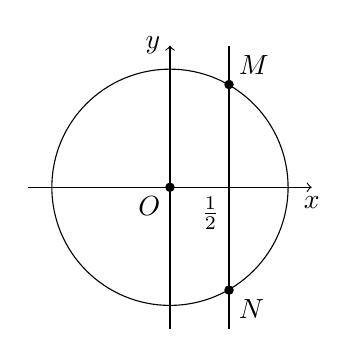
\begin{tikzpicture}[scale=1.5]
\draw[->] (-1.2,0) -- (1.2,0) node[below] {$x$};
\draw[->] (0,-1.2) -- (0,1.2) node[left] {$y$};
\draw (0,0) circle (1);
\draw (0,-1) -- (0,1);
\draw (0,0) node[below left] {$O$};
\draw (1/2,-1.2) -- (1/2,1.2);
\draw (1/2,0) node[below left] {$\frac{1}{2}$};
\draw (1/2,0.87) node[above right] {$M$};
\draw (1/2,-0.87) node[below right] {$N$};
\filldraw (0,0) circle (1pt);
\filldraw (1/2,0.87) circle (1pt);
\filldraw (1/2,-0.87) circle (1pt);
\end{tikzpicture}}
\loigiai{
\begin{itemchoice}
\itemch \textbf{Sai}.\\
Từ phương trình (*), ta có $\cos x=\dfrac{\sqrt{3}}{2}$.\\
Các nghiệm của phương trình là $x=\dfrac{\pi}{6}+k2\pi$ và $x=-\dfrac{\pi}{6}+k2\pi$, $k\in \mathbb{Z}$.\\
Điểm $M$ trên đường tròn lượng giác có hoành độ $\dfrac{1}{2}$ và nằm ở góc phần tư thứ nhất, tương ứng với góc $\dfrac{\pi}{3}$.\\
Điểm $N$ trên đường tròn lượng giác có hoành độ $\dfrac{1}{2}$ và nằm ở góc phần tư thứ tư, tương ứng với góc $-\dfrac{\pi}{3}$.
\itemch \textbf{Đúng}.\\
Chia cả hai vế của phương trình $2\cos x=\sqrt{3}$ cho $2$, ta được $\cos x=\dfrac{\sqrt{3}}{2}$.
\itemch \textbf{Sai}.\\
Phương trình $(*)$ có nghiệm $x=\dfrac{\pi}{6}+k2\pi$ và $x=-\dfrac{\pi}{6}+k2\pi$, $k\in \mathbb{Z}$.\\
Vậy phương trình $(*)$ không có nghiệm $x=\dfrac{\pi}{3}$.
\itemch \textbf{Đúng}.\\
Phương trình $(*)$ có nghiệm $x=\dfrac{\pi}{6}+k2\pi$ và $x=-\dfrac{\pi}{6}+k2\pi$, $k\in \mathbb{Z}$.\\
Nghiệm $x=\dfrac{\pi}{6}+k2\pi$ nằm trong khoảng $\left(0; \dfrac{\pi}{2}\right)$ khi $k=0$.\\
Nghiệm $x=-\dfrac{\pi}{6}+k2\pi$ không nằm trong khoảng $\left(0; \dfrac{\pi}{2}\right)$ với mọi giá trị của $k$.\\
Vậy phương trình $(*)$ chỉ có một nghiệm trong khoảng $\left(0; \dfrac{\pi}{2}\right)$.
\end{itemchoice}
}
\end{ex}

\begin{ex}[THPT Chuyên Bình Thuận 24 - 25]%[1D1V5-6]%[Dự án đề cương 3 Khối NH24-25-Dot1-Nguyễn Sĩ Đạt]
\immini{
Một vật dao động xung quanh vị trí cân bằng theo phương trình $x=1{,}5\cos \left(\dfrac{t\pi}{4} \right)$ (tham khảo hình vẽ); trong đó $t$ là thời gian được tính bằng giây và quãng đường $h=|x|$ được tính bằng mét là khoảng cách theo phương ngang của chất điểm đối với vị trí cân bằng. Khi đó
\choiceTF
{\True Vật ở xa vị trí cân bằng nhất nghĩa là $h=1{,}5$ m}
{Trong $10$ giây đầu tiên, có hai thời điểm vật ở xa vị trí cân bằng nhất}
{\True Khi vật ở vị trí cân bằng thì $\cos \left(\dfrac{t\pi}{4} \right)=0$}
{Trong khoảng từ $0$ đến $20$ giây thì vật đi qua vị trí cân bằng $4$ lần}
}{
\definecolor{darkpastelgreen}{rgb}{0.01, 0.75, 0.24}
\definecolor{almond}{rgb}{0.94, 0.87, 0.8}
\definecolor{arsenic}{rgb}{0.23, 0.27, 0.29}
\definecolor{eggplant}{rgb}{0.38, 0.25, 0.32}
\definecolor{crimson}{rgb}{0.86, 0.08, 0.24}
\begin{tikzpicture}[line join=round, line cap=round,scale=.6,transform shape]
\clip (-2.5,-2.5) rectangle (4.5,4.2);
\tikzset{q_h/.pic={
% Tre
\draw[fill=darkpastelgreen] (-.05,4)--(.9,-1.8)
..controls +(30:.05) and +(-30:.05) ..(1,-1.75)--(.05,4);
\draw[fill=darkpastelgreen] (-.1,4)--(.6,-1.4)
..controls +(30:.05) and +(-30:.05) ..(.5,-1.4)--(-.2,4)
;
%----------------------
\def\M{ 
(-.2,1.76)
..controls +(-80:.1) and +(80:.1) ..(-.18,1.6)
..controls +(-40:.1) and +(30:.06) ..(-.18,1.5)--(-.17,1.46)--(-.22,1.44)--(-.19,1.43)--(-.2,1.43)
..controls +(-80:.1) and +(-12:.05) ..(-.3,1.35)--(-.35,1.28)--(-.55,1.35)
..controls +(60:.1) and +(-90:.05) ..(-.45,1.5)
..controls +(100:.1) and +(140:.05) ..(-.38,1.55)
..controls +(70:.1) and +(-140:.05) ..cycle
;
}

\draw[black]\M;
\fill[almond] \M;
\draw (-.2,1.76)
..controls +(-140:.1) and +(50:.05) ..(-.3,1.6)
(-.2,1.76)
..controls +(-120:.1) and +(40:.05) ..(-.25,1.6)
(-.28,1.578)
..controls +(-20:.02) and +(-150:.02) ..(-.22,1.58)
(-.25,1.568)--(-.23,1.567);
%------------------Áo
\def\A3{ 
(-.1,.9)
..controls +(-30:.05) and +(110:0) ..(.18,1)
--(.19,.95)
..controls +(-140:.05) and +(30:.05) ..(-.1,.7)--cycle
;
}
\fill[arsenic] \A3;
\draw[black]\A3;
\def\A2{ 
(-.35,1.28)
..controls +(-30:.05) and +(110:.05) ..(-.25,1.18)
..controls +(-70:.05) and +(90:.02) ..(-.05,.9)
..controls +(-90:.02) and +(50:.05) ..(-.05,.4)
..controls +(-130:.02) and +(50:.05) ..(.6,-.8)
..controls +(-130:.02) and +(50:.05) ..(.9,-1.8)
..controls +(-130:.2) and +(30:.3) ..(-.5,-2.3)
..controls +(130:.2) and +(-90:.1) ..(-.2,-1.5)
..controls +(130:.2) and +(-140:.1) ..cycle
;
}
\fill[arsenic] \A2;
\draw[black]\A2;
\def\A{ 
(-.55,1.35)
..controls +(-150:.2) and +(120:.1) ..(-.45,0)
..controls +(-60:.1) and +(50:.1) ..(-.3,-1.6)
..controls +(-10:.1) and +(-120:.1) ..(-.15,-1.5)
..controls +(60:.1) and +(-120:.1) ..(0,-1.45)
..controls +(120:.3) and +(-50:.1) ..(-.35,.77)
..controls +(-50:.1) and +(130:.1) ..(-.15,.48)
..controls +(-50:.1) and +(-130:.1) ..(.43,.93)
..controls +(-130:.05) and +(-40:.05) ..(.3,1.05)
..controls +(-130:.05) and +(40:.05) ..(-.05,.75)
..controls +(-140:.05) and +(-40:.05) ..(-.3,1.15)
..controls +(100:.05) and +(-40:.05) ..(-.35,1.28)--cycle
;
}
\fill[eggplant] \A;
\draw[black]\A;
%-------------------------------
%nón
\def\N{ 
(-.14,1.95)
..controls +(-80:.1) and +(80:.1) ..(-.17,1.7)
..controls +(110:.02) and +(-40:.02) ..(-.2,1.76)
..controls +(-110:.1) and +(50:.4) ..(-.48,1.45)--(-.45,1.35)..controls +(-150:.05) and +(20:.05) ..(-.7,1.32)
..controls +(50:.05) and +(-120:.05) ..(-.65,1.45)
..controls +(160:.02) and +(-50:.02) ..(-.7,1.48)
..controls +(160:.02) and +(-50:.02) ..(-.8,1.6)--(-.75,1.63)
..controls +(-20:.06) and +(130:.04) ..(-.6,1.47)
..controls +(130:.2) and +(-90:.1) ..(-.7,1.78)
..controls +(90:.1) and +(170:.1) ..(-.4,1.9)
..controls +(20:.1) and +(160:.1) ..cycle
;
}
\fill[arsenic] \N;
\draw[black]\N;
\draw (-.14,1.95)
..controls +(-100:.05) and +(40:.06) ..(-.2,1.76)
(-.5,1.55)
..controls +(30:.1) and +(-100:.06) ..(-.3,1.76)
(-.6,1.7)
..controls +(-55:.1) and +(120:.06) ..(-.55,1.5)
;

\def\T1{ 
(.3,1.03)
..controls +(60:.05) and +(-120:.05) ..(.35,1.15)
..controls +(60:.05) and +(-140:.05) ..(.45,1.26)
..controls +(30:.05) and +(60:.04) ..(.5,1.22)
..controls +(30:.03) and +(50:.03) ..(.54,1.18)
..controls +(30:.03) and +(50:.03) ..(.56,1.12)
..controls +(30:.03) and +(50:.03) ..(.58,1.07)
..controls +(160:.03) and +(40:.03) ..(.49,1)
..controls +(-140:.03) and +(40:.03) ..(.41,.92)--cycle
;
}
\fill[almond] \T1;
\draw[black]\T1;

\fill[crimson](-.27,.4)
..controls +(-80:.6) and +(-80:.1) ..(-.5,-1.9)--(-.45,-1.85)
..controls +(90:.1) and +(-80:1) ..(-.28,.48)--cycle;

\fill[crimson](-.27,.4)
..controls +(-80:.6) and +(-80:.1) ..(-.2,-1.9)--(-.15,-1.85)
..controls +(90:.1) and +(-80:1) ..(-.28,.48)--cycle;

}}
\tikzset{no/.pic={
\draw[crimson] (1.8,-1)
..controls +(150:.4) and +(-120:.5) ..(1.7,-1)
..controls +(30:.4) and +(-40:.3) ..(1.75,-1)
..controls +(-30:.2) and +(40:.2) ..(1.7,-1.4)
(1.75,-1)
..controls +(-50:.1) and +(20:.1) ..(1.7,-1.2)

;
}}
\draw[thick] (4,-1.25) arc(-60:-120:6cm);
\draw[dashed,thick] (4,-1.25)--(1.3,4)--(-2,-1.25) (1.3,4)--(1.3,-2);
\node at (1.6,.5) [rotate=90]{ Vị trí cân bằng};
\draw[thick,<->] (.35,-2)--(1.3,-2);
\node at (.85,-2) [above]{ $h$};
\fill (4,-1.25) circle (0.05);
\fill (-2,-1.25) circle (0.05);
\fill (1.3,4) circle (0.05);
\path
(0,0)pic[scale=1,rotate=-20]{q_h}(-.88,1.48)pic[scale=1, scale=.7,rotate=-20]{no};

\end{tikzpicture}
}
\loigiai{
\begin{itemchoice}
\itemch \textbf{Đúng}.\\
Ta có $h=|x|= \left|1{,}5 \cos \left(\dfrac{t\pi}{4}\right)\right|\leq 1{,}5$.\\
Vật ở xa vị trí cân bằng nhất nghĩa là $h=1{,}5$ m.
\itemch \textbf{Sai}.\\
Khi đó, $\cos \left( \dfrac{t\pi}{4} \right) = \pm 1 \Leftrightarrow \hoac{& \dfrac{t\pi}{4} = k2\pi\\ & \dfrac{t\pi}{4} = \pi + k2\pi} \Leftrightarrow \hoac{& t=8k\\& t=4+8k}\quad (k \in \mathbb{Z})$.\\
Vậy trong 10 giây đầu tiên thì vật ở xa vị trí cân bằng nhất tại các thời điểm $t=0$, $t=4$, $t=8$ (giây).
\itemch \textbf{Đúng}.\\
Khi vật ở vị trí cân bằng thì  
\begin{eqnarray*}
& & x = 0\\
&\Leftrightarrow & 1{,}5 \cos \left(\dfrac{t\pi}{4}\right)=0\\
&\Leftrightarrow & \cos \left( \dfrac{t\pi}{4} \right)=0\\
&\Leftrightarrow & \dfrac{t\pi}{4} = \dfrac{\pi}{2}+k\pi \Rightarrow t=2+4k\quad (k \in \mathbb{Z}).
\end{eqnarray*}
\itemch \textbf{Sai}.\\
Trong khoảng từ $0$ đến $20$ giây thì vật ở vị trí cân bằng tại các thời điểm $t=2$, $t=6$, $t=10$, $t=14$, $t=18$ (giây); tức là có $5$ lần vật qua vị trí cân bằng.
\end{itemchoice}
}
\end{ex}

\Closesolutionfile{ans}

\ind{PHẦN III.} \inden{Trả lời ngắn}\\
\setcounter{ex}{0}
\Opensolutionfile{ans}[ans/2D1-Bai1-DS]%--Đặt tên 2D1-Bai1-DS

\begin{ex}[Sở Bắc Giang 24 - 25]%[1D1V5-6]%[Dự án đề cương 3 Khối NH24-25-Dot1-Nguyễn Sĩ Đạt]
Hằng ngày, mực nước của một con kênh lên xuống theo thủy triều. Độ sâu $h$ (m) của mực nước trong kênh đó tính theo thời gian $t$ giờ được cho bởi công thức $h = 2\cos\left(\dfrac{\pi t}{12} + \dfrac{\pi}{3}\right) + 12$ với ($0 \leq t \leq 24$). Độ sâu của mực nước trong con kênh đó đạt $14$ m lần đầu tiên trong ngày vào lúc mấy giờ?
\shortans{$20$}
\loigiai{
Khi độ sau của mực nước là $14$ m, ta có
\begin{eqnarray*}
h&=&14 \\
2\cos\left(\dfrac{\pi t}{12} + \dfrac{\pi}{3}\right) + 12&=&14 \\
\cos\left(\dfrac{\pi t}{12} + \dfrac{\pi}{3}\right) &=& 1 \\
\dfrac{\pi t}{12} + \dfrac{\pi}{3} &=& k2\pi \\
t &=&-4+24k\quad (k\in\mathbb{Z}).
\end{eqnarray*}
Ta có $0\leq t \leq 24$ nên $0\leq -4+24k \leq 24$, suy ra $\dfrac{1}{6}\leq t \leq \dfrac{7}{6}$.\\
Do $t\in\mathbb{Z}$ nên $t=1$.\\
Vậy độ sâu của mực nước trong con kênh đó đạt $14m$ lần đầu tiên trong ngày vào lúc $t=-4+24\cdot1=20$ giờ.
}
\end{ex}

\begin{ex}[THPT Tân Châu - An Giang 24 - 25]%[1D1V5-6]%[Dự án đề cương 3 Khối NH24-25-Dot1-Nguyễn Sĩ Đạt]
Số giờ có ánh sáng mặt trời của một thành phố A ở vĩ độ $40^\circ$ Bắc trong ngày thứ $t$ của một năm không nhuận được cho bởi hàm số có công thức
$d(t)=3\sin \left[\dfrac{\pi}{182} (t-80) \right]+12$,
với $t \in \mathbb{Z}$ và $0< t \le 365$. Biết rằng vào một ngày của tháng $6$ dương lịch trong năm đó thì thành phố A có đúng $15$ giờ có ánh sáng mặt trời. Hỏi ngày đó là ngày mấy của tháng $6$?
\shortans{$20$}
\loigiai{
Giả sử thành phố A có đúng $15$ giờ có ánh sáng mặt trời vào ngày thứ $\mathrm{t}_0$.\\
Ta có $d(t_0)=3 \sin \left[\dfrac{\pi}{182}\left(t_0-80\right)\right]+12$.\\
Mà $d(t_0)=15$ nên ta có
\begin{eqnarray*}
&& 3 \sin \left[\dfrac{\pi}{182}(t_0-80)\right]+12=15 \\
& \Leftrightarrow& 3 \sin \left[\dfrac{\pi}{182}(t_0-80)\right]=3\\
& \Leftrightarrow& \sin \left[\dfrac{\pi}{182}(t_0-80)\right]=1\\
& \Leftrightarrow& \dfrac{\pi}{182}(t_0-80)=\dfrac{\pi}{2}+k2\pi, k \in \mathbb{Z} \\
& \Leftrightarrow& t_0-80=91+364k, k \in \mathbb{Z} \\
& \Leftrightarrow& t_0=364k+171, k \in \mathbb{Z}.
\end{eqnarray*}
Mà $0 < t_0 \leq 365 \Leftrightarrow -171 < 364k \leq 194\Leftrightarrow -\dfrac{171}{364} < k \leq \dfrac{97}{182}$.\\
Mà $k \in \mathbb{Z}$ nên $k=0$ do đó $t_0=171$.\\
Vậy thành phố A có đúng $15$ giờ có ánh sáng mặt trời vào ngày thứ $171$ trong năm tức là vào ngày thứ $20$ của tháng $6$.
}
\end{ex}



\begin{ex}[THPT Tây Thạnh - TPHCM 24 - 25]%[1D1C5-6]%[Dự án đề cương 3 Khối NH24-25-Dot1-Nguyễn Sĩ Đạt]
\immini{Giả sử một con tàu vũ trụ được phóng lên từ mũi Canaveral ở Mĩ. Nó chuyển động theo một quỹ đạo được mô tả trên một bản đồ phẳng (quanh đường xích đạo) của mặt đất như hình mô phỏng bên dưới. Điểm $M$ mô tả cho con tàu, đường thẳng $\Delta$ mô tả cho đường xích đạo. Khoảng cách $h$ (km) từ $M$ đến $\Delta$ được tính theo công thức $h=|d|$, trong đó $d=4000\cos\left[\dfrac{\pi}{45}(t-10)\right]$, với $t$ (phút) là thời gian trôi qua kể từ khi con tàu đi vào quỹ đạo, $d>0$ nếu $M$ ở phía trên $\Delta$, $d<0$ nếu $M$ ở phía dưới $\Delta$. Hãy tìm thời điểm sớm nhất sau khi con tàu đi vào quỹ đạo để có $d$ lớn nhất.}
{\begin{tikzpicture}[line width=2pt,font=\footnotesize, line join=round, line cap=round, >=stealth,scale = .5]
\fill[blue!20](-5,-5)rectangle(5,2.6);
\fill[teal!50!green](-4.65,0)..controls++(45:0.5)and++(160:0.75)..(-3.9,0)--++(-60:0.5)--++(-91:0.5)--++(-45:0.75)--++(-90:0.15)--++(-25:0.85)--++(-90:0.2)--++(-95:0.35)--++(0:0.1)--++(-100:0.2)--++(-50:0.35)--++(-170:0.1)--++(-92:1.35)--++(-5:0.2)--++(30:0.1)--++(88:0.45)--++(70:0.1)--++(60:0.3)--++(5:0.1)--++(50:0.2)--++(62:0.2)--++(50:0.2)--++(88:0.3)--++(40:0.2)--++(88:0.1)--++(130:0.2)--++(160:0.25)--++(134:0.15)--++(85:0.1)--++(170:0.2)--++(150:0.2)--++(175:0.2)--++(155:0.1)--++(160:0.1)--++(145:0.2)--++(150:0.1)--++(90:0.2)--++(-135:0.2)--++(140:0.2)--++(90:0.2)--++(40:0.1)--++(0:0.1)--++(30:0.2)--++(-88:0.2)--++(75:0.3)--++(20:0.2)--++(92:0.2)--++(35:0.2)--++(90:0.1)--++(0:0.15)--++(70:0.2)--++(140:0.2)--++(30:0.1)--++(-20:0.1)--++(40:0.2)--++(145:0.3)--++(90:0.2)--++(-140:0.2)--++(140:0.3)--++(-98:0.55)--++(135:0.2)--++(155:0.2)--++(110:0.3)--++(45:0.4)--++(140:0.5)--++(40:0.1)--++(-35:0.4)--++(90:0.1)--++(-30:0.3)--++(-95:0.2)--++(0:0.2)--++(90:0.2)--++(120:0.2)--++(170:0.3)--++(70:0.55)--++(90:0.1)--++(25:0.2)--++(-90:0.1)--++(-135:0.1)--++(-50:0.2)--++(0:0.2)--++(-75:0.3)--++(-90:0.1)--++(-80:0.2)--++(-70:0.45)--++(-10:0.15)--++(70:0.3)--++(60:0.2)--++(0:0.2)--++(60:0.3)--++(160:0.1)--++(70:0.1)--++(-20:0.1)--++(82:0.5)--++(20:0.15)--++(100:0.1)--++(-170:0.2)--++(65:0.2)--++(-170:0.2)--++(170:0.2)--++(160:0.15)--++(-145:0.3)--++(-175:0.4)--++(90:0.1)--++(-165:0.75)--++(-90:0.2)--++(-40:0.2)--++(-160:0.2)--++(-170:0.5)--++(-90:0.5)--++(130:0.2)--++(-182:0.5)--++(-150:0.2)--++(160:0.5)--++(-175:0.2)--++(-140:0.2)--++(-90:0.2)--++(-10:0.1)--++(-90:0.2)--++(-70:0.2)--cycle;
\fill[teal!60!green](0,-0.8)--++(178:0.2)--++(-170:0.2)--++(-130:0.2)--++(-110:0.3)--++(-115:0.2)--++(-86:0.4)--++(-20:0.2)--++(-88:0.1)--++(-30:0.2)--++(40:0.2)--++(-30:0.3)--++(-92:0.1)--++(-80:0.4)--++(-92:0.3)--++(-45:0.2)--++(-85:0.4)--++(25:0.3)--++(60:0.4)--++(100:0.2)--++(30:0.2)--++(90:0.4)--++(60:0.6)--++(135:0.1)--++(180:0.2)--++(130:0.1)--++(115:0.6)--++(-40:0.5)--++(-90:0.1)--++(20:0.4)--++(120:0.2)--++(-140:0.1)--++(130:0.2)--++(0:0.3)--++(-40:0.4)--++(-70:0.4)--++(55:0.65)--++(-80:0.3)--++(10:0.2)--++(-80:0.2)--++(0:0.1)--++(95:0.1)--++(-40:0.15)--++(20:0.2)--++(115:0.3)--++(20:0.3)--++(80:0.2)--++(0:0.1)--++(110:0.4)--++(90:0.2)--++(-25:0.1)--++(-80:0.25)--++(0:0.15)--++(80:0.3)--++(0:0.1)--++(70:0.5)--++(130:0.2)--++(65:0.3)--++(10:0.3)--++(80:0.1)--++(0:0.3)--++(-90:0.1)--++(25:0.4)--++(90:0.1)--++(30:0.1)--++(-20:0.2)--++(90:0.2)--++(170:0.4)--++(180:0.3)--++(160:0.2)--++(165:0.4)--++(-160:0.3)--++(150:0.2)--++(165:0.2)--++(180:0.3)--++(50:0.2)--++(140:0.3)--++(-150:0.4)--++(-150:0.3)--++(-130:0.5)--++(-170:0.75)--++(-130:0.3)--++(130:0.2)--++(40:0.2)--++(150:0.3)--++(190:0.3)--++(-110:0.4)--++(180:0.2)--++(-90:0.2)--++(0:0.2)--++(-90:0.1)--++(40:0.2)--++(90:0.2)--++(60:0.2)--++(-90:0.3)--++(-20:0.2)--++(-140:0.4)--++(180:0.3)--++(-130:0.3)--++(-92:0.3)--++(180:0.2)--++(-90:0.2)--++(0:0.2)--++(45:0.3)--++(-45:0.3)--++(45:0.1)--++(130:0.2)--++(30:0.2)--++(-50:0.3)--++(-30:0.3)--++(-90:0.2)--++(175:0.5)--cycle;
\fill[teal!60!green](3,-3)--++(80:0.2)--++(0:0.1)--++(85:0.2)--++(30:0.2)--++(20:0.2)--++(-45:0.2)--++(60:0.15)--++(-40:0.3)--++(-60:0.3)--++(-90:0.1)--++(-30:0.1)--++(-100:0.4)--++(-145:0.1)--++(-90:0.2)--++(130:0.3)--++(170:0.2)--++(90:0.2)--++(160:0.2)--++(-130:0.3)--++(180:0.2)--++(90:0.2)--cycle;
\draw[blue](-2.5,-1.3)..controls++(50:3)and++(-140:3)..(5,-3)coordinate[pos=0.2](M);
\fill[red](M)circle(3pt)node[above]{\textbf{M}};
\path(M)node[below=2mm,scale=1.25,red]{\textbf{Canaveral}};
\draw[dashed,] (-5,-2.2)--(5,-2.2);
\path(3.5,-2.3)node[above=0mm,scale=1.25]{\textbf{Xích đạo}};
\end{tikzpicture}}
\shortans[]{$10$}
\loigiai
{\begin{itemize}
\item Trường hợp 1: Xét $M$ ở phía trên $\Delta$, khi đó thời điểm tàu đi vào quỹ đạo có $d=4000$ là lớn nhất với điều kiện 
$$\cos\left[\dfrac{\pi}{45}(t-10)\right]=1\Leftrightarrow \dfrac{\pi}{45}(t-10)=k2\pi\Leftrightarrow t=10+90k, k\in\mathbb{Z}.$$
Do $t>0$ nên thời điểm sớm nhất trong trường hợp này là $t=10$ (phút).
\item Trường hợp 2: Xét $M$ ở phía dưới $\Delta$, khi đó thời điểm tàu đi vào quỹ đạo khi $d=-4000$ thì $h$ là lớn nhất với điều kiện 
$$\cos\left[\dfrac{\pi}{45}(t-10)\right]=-1\Leftrightarrow \dfrac{\pi}{45}(t-10)=\pi+k2\pi\Leftrightarrow t=55+90k, k\in\mathbb{Z}.$$
Do $t>0$ nên thời điểm sớm nhất trong trường hợp này là $t=55$ (phút).
\end{itemize}
Vậy sau $10$ phút kể từ khi con tàu đi vào quỹ đạo thì có $d$ lớn nhất.
}
\end{ex}

\begin{ex}[Chuyên Hùng Vương - Phú Thọ 24 - 25]%[1D1C5-6]%[Dự án đề cương 3 Khối NH24-25-Dot1-Nguyễn Sĩ Đạt]
Một quả bóng được ném xiên một góc $\alpha\left(0^{\circ} < \alpha < 90^{\circ}\right)$ từ mặt đất với tốc độ $v_0$ (m/s). Khoảng cách theo phương ngang từ vị trí ban đầu của quả bóng đến vị trí bóng chạm đất được tính theo công thức $d=\dfrac{v_0^2\sin 2\alpha}{10}$. Nếu tốc độ ban đầu của quả bóng là $10$ m/s thì tồn tại hai góc ném $\alpha_1$, $\alpha_2$ $\left(\alpha_1 > \alpha_2\right)$ để khoảng cách $d$ là $5$ m. Hiệu số đo hai góc ném $\alpha_1-\alpha_2$ bằng bao nhiêu độ?
\shortans{$60$}
\loigiai{
Theo giả thuyết bài toán ta có 
$$\dfrac{10^2\cdot \sin 2\alpha}{10}=5\Leftrightarrow\sin 2\alpha=\dfrac{1}{2}\Leftrightarrow\heva{&2\alpha =30^\circ + k360^\circ\\&2\alpha=150^\circ+k360^\circ}\Leftrightarrow\heva{&\alpha =15^\circ + k180^\circ\\&\alpha=75^\circ+k180^\circ}\,(k\in\mathbb{Z}).$$
Vì $0^{\circ} < \alpha < 90^{\circ}$ và $\alpha_1 > \alpha_2$ nên $\alpha_1=75^\circ$, $\alpha_2=15^\circ$.\\
Suy ra $\alpha_1-\alpha_2=75^\circ-15^\circ=60^\circ$.
}
\end{ex}

\begin{ex}%[Vu Long]%[1D1H5-6]
	\immini
	{Trong môn cầu lông, khi phát cầu, người chơi cần đánh cầu qua khỏi lưới sang phía sân đối phương và không được để cho cầu rơi ngoài biên. Trong mặt phẳng tọa độ $Oxy$, chọn điểm có tọa độ $(0; y_0)$ là điểm xuất phát thì phương trình quỹ đạo của cầu lông khi rời khỏi mặt vợt là $y = \dfrac{-g \cdot x^2}{2v_0^2\cos^2\alpha} + x\cdot \tan\alpha + y_0$.}
	{\begin{tikzpicture}[line cap=round,line join=round,>=stealth]
			\def\caulong{\begin{tikzpicture}[line cap=round,line join=round]
					\definecolor{cdde8e8}{RGB}{221,232,232}
					\definecolor{cc8b7b7}{RGB}{200,183,183}
					\definecolor{ce8f9f9}{RGB}{232,249,249}
					\clip (9.5,1.15) rectangle +(1.5,1.05);
					\begin{scope}[cm={0.67,0,0,0.67,(0,0)}]
						\path[fill=cdde8e8] (16.38,1.91) .. controls +(-0.01,0.07) and +(0.08,-0.02) .. (16.23,2.06) .. controls +(0.07,0.04) and +(0.01,-0.07) .. (16.33,2.24) .. controls +(-0.01,0.07) and +(0.08,-0.01) .. (16.17,2.38) .. controls +(0.06,0.04) and +(0.02,-0.07) .. (16.25,2.56) .. controls +(-0.02,0.07) and +(0.08,-0.01) .. (16.09,2.68) .. controls +(0.06,0.05) and +(0.03,-0.07) .. (16.15,2.87) .. controls +(-0.03,0.07) and +(0.08,0) .. (15.97,2.97) .. controls +(0.06,0.06) and +(0.04,-0.07) .. (16.03,3.19) .. controls +(-0.05,0.09) and +(0.1,0.06) .. (15.75,3.18) -- (15.31,2.9) .. controls +(-0.05,-0.03) and +(0.01,0.04) .. (15.19,2.77) -- (14.58,2.42) -- (14.75,1.81) -- (14.75,1.81) -- (15.46,1.83) .. controls +(0.03,-0.02) and +(-0.06,0) .. (15.62,1.78) -- (16.14,1.77) .. controls +(0.12,-0) and +(0.01,-0.1) .. (16.38,1.91) -- cycle (15.78,2) .. controls +(-0.11,-0.02) and +(0.07,0.1) .. (15.46,1.88) -- (15.36,1.88) .. controls +(-0.01,0.05) and +(0.01,-0.06) .. (15.33,2.05) -- (15.41,2.06) .. controls +(0.09,-0.1) and +(-0.12,-0.01) .. (15.78,2) -- cycle (15.11,2.27) .. controls +(-0.01,0.05) and +(0.02,-0.05) .. (15.06,2.42) -- (15.17,2.46) .. controls +(0.02,-0.05) and +(-0.01,0.05) .. (15.22,2.3) -- cycle (15.04,2.47) .. controls +(-0.01,0.04) and +(0.02,-0.04) .. (14.99,2.6) -- (15.09,2.66) .. controls +(0.02,-0.05) and +(-0.02,0.05) .. (15.15,2.51) -- cycle (15,2.45) -- (14.9,2.41) .. controls +(-0.01,0.04) and +(0.01,-0.04) .. (14.86,2.53) -- (14.95,2.58) .. controls +(0.02,-0.04) and +(-0.01,0.04) .. (15,2.45) -- cycle (15.01,2.4) .. controls +(0.02,-0.05) and +(-0.01,0.05) .. (15.06,2.26) -- (14.96,2.23) .. controls +(-0.01,0.05) and +(0.01,-0.04) .. (14.92,2.36) -- cycle (15.07,2.2) .. controls +(0.01,-0.05) and +(-0.01,0.05) .. (15.11,2.06) -- (15.01,2.04) .. controls +(-0.01,0.04) and +(0.01,-0.05) .. (14.97,2.18) -- cycle (15.12,2.22) -- (15.23,2.25) .. controls +(0.01,-0.05) and +(-0.01,0.05) .. (15.27,2.09) -- (15.16,2.07) .. controls +(-0.01,0.05) and +(0.01,-0.05) .. (15.12,2.22) -- cycle (15.28,2.04) .. controls +(0.01,-0.05) and +(-0.01,0.05) .. (15.31,1.88) -- (15.19,1.88) .. controls +(-0.01,0.05) and +(0.01,-0.04) .. (15.17,2.02) -- cycle (15.71,2.27) .. controls +(-0.1,-0.03) and +(0.05,0.11) .. (15.41,2.11) -- (15.32,2.09) .. controls +(-0.01,0.06) and +(0.01,-0.05) .. (15.28,2.26) -- (15.36,2.29) .. controls +(0.1,-0.08) and +(-0.11,-0.02) .. (15.71,2.27) -- cycle (15.64,2.53) .. controls +(-0.1,-0.04) and +(0.04,0.12) .. (15.34,2.33) -- (15.27,2.31) .. controls +(-0.02,0.05) and +(0.02,-0.05) .. (15.21,2.48) -- (15.3,2.51) .. controls +(0.1,-0.07) and +(-0.11,-0.03) .. (15.64,2.53) -- cycle (15.27,2.56) -- (15.2,2.53) .. controls +(-0.02,0.05) and +(0.02,-0.05) .. (15.13,2.68) -- (15.22,2.73) .. controls +(0.12,-0.04) and +(-0.11,-0.04) .. (15.58,2.8) .. controls +(-0.1,-0.06) and +(0.02,0.14) .. (15.27,2.56) -- cycle (15.02,1.99) -- (15.12,2.01) .. controls +(0.01,-0.04) and +(-0.01,0.04) .. (15.14,1.88) -- (15.04,1.87) .. controls +(-0.01,0.04) and +(0.01,-0.04) .. (15.02,1.99) -- cycle;
						\path[fill=cdde8e8] (14.67,2.47) -- (14.47,2.42) .. controls +(-0.18,-0.05) and +(-0.05,0.18) .. (14.23,2) .. controls +(0.05,-0.18) and +(-0.18,-0.05) .. (14.65,1.76) -- (14.85,1.82) -- cycle;
					\end{scope}
					
					\path[fill=ce8f9f9,line width=0.02] (13.85,3.13) .. controls +(0.01,-0.03) and +(0.04,0.01) .. (13.8,3.06) .. controls +(-0.04,-0.01) and +(0.01,-0.03) .. (13.72,3.09) .. controls +(-0.01,0.03) and +(-0.04,-0.01) .. (13.77,3.16) .. controls +(0.04,0.01) and +(-0.01,0.03) .. (13.85,3.13) -- cycle;
					\begin{scope}[opacity=0.1,cm={0.67,0,0,0.67,(0,0)},transparency group]
						\path[fill=cc8b7b7,] (16.38,1.91) .. controls +(-0.01,0.07) and +(0.08,-0.02) .. (16.23,2.06) .. controls +(0.06,0.04) and +(0,-0.07) .. (16.33,2.23) .. controls +(-0.26,-0.1) and +(0.23,0.05) .. (15.59,1.99) .. controls +(0.07,0) and +(-0.07,-0) .. (15.78,2) .. controls +(-0.11,-0.02) and +(0.07,0.1) .. (15.46,1.88) -- (15.36,1.88) .. controls +(-0,0.02) and +(0,-0.02) .. (15.35,1.94) .. controls +(-0.02,-0) and +(0.02,0) .. (15.3,1.94) .. controls +(0,-0.02) and +(-0,0.02) .. (15.31,1.88) -- (15.19,1.88) .. controls +(-0,0.01) and +(0,-0.01) .. (15.19,1.92) .. controls +(-0.02,0) and +(0.02,0) .. (15.13,1.92) .. controls +(0,-0.01) and +(-0,0.01) .. (15.14,1.88) -- (15.04,1.87) .. controls +(-0,0.01) and +(0,-0.01) .. (15.04,1.91) .. controls +(-0.23,-0.01) and +(-0.03,-0.4) .. (14.3,2.31) .. controls +(-0.07,-0.08) and +(-0.03,0.11) .. (14.23,2) .. controls +(0.05,-0.18) and +(-0.18,-0.05) .. (14.65,1.76) .. controls +(0.09,0.03) and +(-0.09,-0.01) .. (14.91,1.81) -- (15.46,1.83) .. controls +(0.17,-0.09) and +(-0.2,0.01) .. (16.14,1.77) .. controls +(0.12,-0) and +(0.01,-0.1) .. (16.38,1.91) -- cycle;
					\end{scope}
					\begin{scope}[cm={0.67,0,0,0.67,(0,0)}]
						\path[fill=red,] (14.79,1.79) -- (14.91,1.81) -- (14.72,2.51) -- (14.6,2.46) -- (14.79,1.79)-- cycle;
					\end{scope}
			\end{tikzpicture}}
			
			\draw[->] (-0.5,0)--(7,0);
			\draw[->] (0,-0.5)--(0,2);
			\draw[gray]  (6,0) coordinate (A) .. controls +(153:1.46) and +(-2:1.06) .. (1.87,1.76) coordinate (B) .. controls +(178:0.25) and +(21:0.2) .. (1.18,1.65) coordinate (C) .. controls +(-159:0.55) and +(52:0.45) .. (0,0.71) coordinate (D);
			\draw[->]  (D) -- (0.76,1.28);
			\path ($(C)+(0,0.03)$) node[rotate=10]{\resizebox{!}{0.2cm}{\caulong}};
			\foreach \diem/\goc in {A/-90,D/180}{
				\fill (\diem) circle (1pt) node[shift={(\goc:7pt)},font=\scriptsize]{$\diem$};
			}
	\end{tikzpicture}}
	\noindent
	Trong đó
	\begin{itemize}
		\item $g$ là gia tốc trọng trường (thường được chọn là $9{,}8$ m/s$^2$);
		\item $\alpha$ là góc phát cầu (so với phương ngang của mặt đất);
		\item $v_0$ là vận tốc ban đầu của cầu;
		\item $y_0$ là khoảng cách từ vị trí phát cầu đến mặt đất.
	\end{itemize}
	Đây là một hàm số bậc hai nên quỹ đạo chuyển động của cầu lông là một parabol. Một người chơi cầu lông đang đứng, khoảng cách từ vị trí người này đến vị trí cầu rơi chạm đất (tầm bay xa) là $6{,}68$ m. Quan sát hình vẽ trên, hỏi người chơi đã phát cầu góc khoảng bao nhiêu độ so với mặt đất? Biết cầu rời mặt vợt ở độ cao $0{,}7$ m so với mặt đất; vận tốc xuất phát của cầu là $8$ m/s; người chơi không phát cầu quá $50^\circ$ và bỏ qua sức cản của gió, xem quỹ đạo của cầu luôn nằm trong mặt phẳng phẳng đứng (\textit{kết quả làm tròn đến hàng đơn vị của độ}).
	\shortans[oly]{30}
	\loigiai{
		Với $g = 9{,}8$ m/s$^2$, vận tốc ban đầu $v_0 = 8$ m/s, phương trình quỹ đạo của cầu
		$$y = \dfrac{-g\cdot x^2}{2v_0^2\cdot \cos^2\alpha} + \tan \alpha\cdot x + y_0$$
		Khoảng cách từ vị trí người này đến vị trí cầu rơi chạm đất (tầm bay xa) là $6{,}68$ m; nghĩa là $x = 6{,}68$ m.\\
		Ta có
		\begin{align*}
			\dfrac{-9{,}8\cdot (6{,}68)^2}{128\cdot \cos^2\alpha} + \tan \alpha\cdot (6{,}68) + 0{,}7 = 0 &\Leftrightarrow \dfrac{-9{,}8\cdot (6{,}68)^2}{128}(1+\tan^2\alpha) + \tan \alpha\cdot (6{,}68) + 0{,}7 = 0\\
			&\Leftrightarrow \hoac{&\tan\alpha \approx 1{,}378\\&\tan\alpha \approx 0{,}576} \Leftrightarrow \hoac{&\alpha \approx 54^\circ\\&\alpha \approx 30^\circ.}
		\end{align*}
		Vậy người chơi đã phát cầu một góc $30^\circ$ so với mặt đất.
	}
\end{ex}
\Closesolutionfile{ans}


\ind{PHẦN IV.} \inden{Tự luận.}\\
\setcounter{ex}{0}

\begin{ex}[THPT NTMK - TPHCM 24-25]%[1D1H5-34]%[Dự án đề cương 3 Khối NH24-25-Dot1-Nguyễn Sĩ Đạt]
Giải các phương trình sau
\begin{multicols}{3}
\begin{enumerate}
\item $\sin 2 x=\sin \dfrac{\pi}{5}$.
\item $\cot \left(x+50^{\circ}\right)=\sqrt{3}$.
\item $\cos \left(3 x-\dfrac{\pi}{4}\right)=\cos 2 x$.
\end{enumerate}
\end{multicols}
\loigiai{
\begin{enumerate}
\item  $\sin 2 x=\sin \dfrac{\pi}{5}$\\
$
\Leftrightarrow \hoac{ 
& 2 x = \dfrac { \pi } { 5 } + k 2 \pi  \\
& 2 x = \pi - \dfrac { \pi } { 5 } + k 2 \pi 
} \Leftrightarrow 
\hoac{
& x=\dfrac{\pi}{10}+k \pi \\
& x=\dfrac{2 \pi}{5}+k \pi
} (k \in \mathbb{Z})
$.
\item 
$  \cot \left(x+50^{\circ}\right)=\sqrt{3} \\
\Leftrightarrow \cot \left(x+50^{\circ}\right)=\cot 30^{\circ} \\
\Leftrightarrow x+50^{\circ}=30^{\circ}+k 180^{\circ} \\
\Leftrightarrow x=-20^{\circ}+k 180^{\circ} \quad(k \in \mathbb{Z})
$.
\item $
\cos \left(3 x-\dfrac{\pi}{4}\right)=\cos 2 x \\
\Leftrightarrow \hoac{
& 3 x - \dfrac { \pi } { 4 } = 2 x + k 2 \pi  \\
& 3 x - \dfrac { \pi } { 4 } = - 2 x + k 2 \pi 
} \Leftrightarrow \hoac{
& x=\dfrac{\pi}{4}+k 2 \pi \\
& x=\dfrac{\pi}{20}+k \dfrac{2 \pi}{5}
} (k \in \mathbb{Z})
$.
\end{enumerate}
}
\end{ex}

\begin{ex}[THPT Bà Điểm - TPHCM 24-25]%[1D1H5-35]%[Dự án đề cương 3 Khối NH24-25-Dot1-Nguyễn Sĩ Đạt]
Giải các phương trình sau
\begin{listEX}[3]
\item $\cos \left(x+\dfrac{5\pi}{6}\right)=-1$; 
\item $\sin \left(2x-\dfrac{\pi}{6}\right)-\cos x =0$; 
\item $\cos^2 3x+\cos^2 5x =1$.
\end{listEX}
\loigiai{ 
\begin{listEX}[1]
\item $\cos \left(x+\dfrac{5\pi}{6}\right)=-1$.\\
Ta có 
\[\cos \left(x+\dfrac{5\pi}{6}\right)=-1\Leftrightarrow x+\dfrac{5\pi}{6} =\pi +k2\pi\Leftrightarrow x =\dfrac{\pi}{6}+k2\pi, \ k \in \mathbb{Z}.\]
Vậy phương trình đã cho  có nghiệm  $x =\dfrac{\pi}{6}+k2\pi, \ k \in \mathbb{Z}$.
\item $\sin \left(2x-\dfrac{\pi}{6}\right)-\cos x =0$.\\
Ta có 
\begin{eqnarray*}
\sin \left(2x-\dfrac{\pi}{6}\right)-\cos x =0
&\Leftrightarrow&\sin \left(2x-\dfrac{\pi}{6}\right)=\cos x\\
&\Leftrightarrow& \sin \left(2x-\dfrac{\pi}{6}\right)=\sin\left(\dfrac{\pi}{2}-x\right)\\
&\Leftrightarrow& \hoac{&2x-\dfrac{\pi}{6}=\dfrac{\pi}{2}-x+k2\pi\\&2x-\dfrac{\pi}{6}=\pi-\dfrac{\pi}{2}+x+k2\pi}\\
&\Leftrightarrow &\hoac{&x=\dfrac{2\pi}{9}+\dfrac{k2\pi}{3}\\&x=\dfrac{2\pi}{3}+k2\pi}, \ k \in \mathbb{Z}.
\end{eqnarray*}
Vậy phương trình đã cho có nghiệm $x=\dfrac{2\pi}{9}+\dfrac{k2\pi}{3}, \ k \in \mathbb{Z} $ và $x=\dfrac{2\pi}{3}+k2\pi, \ k \in \mathbb{Z}$.
\item $\cos^2 3x+\cos^2 5x =1$.\\
Ta có 
\begin{eqnarray*}
\cos^2 3x+\cos^2 5x =1 &\Leftrightarrow& \dfrac{1+\cos 6x}{2}+\dfrac{1+\cos 10x}{2}=1\\
&\Leftrightarrow& \cos 6x +\cos 10=0\\
&\Leftrightarrow& \cos 6x = \cos \left(\pi -10x\right)\\
&\Leftrightarrow& \hoac{&6x=\pi-10x+k2\pi\\&6x=-\pi+10x+k2\pi}\\
&\Leftrightarrow&\hoac{&x=\dfrac{\pi}{16}+\dfrac{k\pi}{8}\\&x=\dfrac{\pi}{4}-\dfrac{k\pi}{2}}, \ k \in \mathbb{Z}.
\end{eqnarray*}
Vậy phương trình đã cho có nghiệm $x=\dfrac{\pi}{16}+\dfrac{k\pi}{8},\ k \in \mathbb{Z}$ và $ x=\dfrac{\pi}{4}-\dfrac{k\pi}{2}, \ k \in \mathbb{Z}$.
\end{listEX}
}
\end{ex}

\begin{ex}[THPT Gia Định - TPHCM 24-25]%[1D1H5-3]%[Dự án đề cương 3 Khối NH24-25-Dot1-Nguyễn Sĩ Đạt]
Tính tổng các nghiệm thuộc nửa khoảng $(-2;3]$ của phương trình $\cos^2x=\dfrac{1}{2}$.
\loigiai{
Ta có $\cos ^2x=\dfrac{1}{2} \Leftrightarrow \cos 2x=0 \Leftrightarrow 2x=\dfrac{\pi}{2}+k\pi \Leftrightarrow x=\dfrac{\pi}{4}+k\dfrac{\pi}{2}$, $k\in \mathbb{Z}$.\\
Trên nửa khoảng $(-2;3]$ ta có các nghiệm thỏa mãn $$-2 <\dfrac{\pi}{4}+k\dfrac{\pi}{2} \leq 3 \Leftrightarrow \dfrac{-8-\pi}{2\pi}<k \leq \dfrac{12-\pi}{2\pi}.$$
Do $k \in \mathbb{Z}$ nên $k \in \{-1;0;1\}$.\\
\begin{itemize}
\item Với $k=-1$ suy ra $x=-\dfrac{\pi}{4}$.
\item Với $k=0$ suy ra $x=\dfrac{\pi}{4}$.
\item Với $k=1$ suy ra $x=\dfrac{3\pi}{4}$.
\end{itemize}
Khi đó ta có tổng các nghiệm $S=-\dfrac{\pi}{4}+\dfrac{\pi}{4}+\dfrac{3\pi}{4}=\dfrac{3\pi}{4}$.
}
\end{ex}
\begin{ex}[THPT Chuyên Hùng Vương - Phú Thọ 24-25]%[1D1V5-6]%[Dự án đề kiểm tra Toán khối 11 học kì 1 NH24-25-Dot 5-Thái Bảo ]
	Một quả bóng được ném xiên một góc $\alpha\left(0^{\circ} < \alpha < 90^{\circ}\right)$ từ mặt đất với tốc độ $v_0$ (m/s). Khoảng cách theo phương ngang từ vị trí ban đầu của quả bóng đến vị trí bóng chạm đất được tính theo công thức $d=\dfrac{v_0^2\sin 2\alpha}{10}$. Nếu tốc độ ban đầu của quả bóng là $10$ m/s thì tồn tại hai góc ném $\alpha_1$, $\alpha_2$ $\left(\alpha_1 > \alpha_2\right)$ để khoảng cách $d$ là $5$ m. Tìm hiệu số đo hai góc ném $\alpha_1-\alpha_2$.
	\loigiai{
		Theo giả thuyết bài toán ta có 
		$$\dfrac{10^2\cdot \sin 2\alpha}{10}=5\Leftrightarrow\sin 2\alpha=\dfrac{1}{2}\Leftrightarrow\heva{&2\alpha =30^\circ + k360^\circ\\&2\alpha=150^\circ+k360^\circ}\Leftrightarrow\heva{&\alpha =15^\circ + k180^\circ\\&\alpha=75^\circ+k180^\circ}\,(k\in\mathbb{Z}).$$
		Vì $0^{\circ} < \alpha < 90^{\circ}$ và $\alpha_1 > \alpha_2$ nên $\alpha_1=75^\circ$, $\alpha_2=15^\circ$.\\
		Suy ra $\alpha_1-\alpha_2=75^\circ-15^\circ=60^\circ$.
	}
\end{ex}
\begin{ex}[THPT Trần Khai Nguyên - TPHCM 24-25]%[Dự án đề cương 3 Khối NH24-25-Dot1-Nguyễn Sĩ Đạt]
Chiều cao $h$ mét của một cabin trên vòng quay vào thời điểm $t$ giây sau khi bắt đầu chuyển động được cho bởi công thức $h(t)=25+20\sin\left(\dfrac{\pi}{30}t+\dfrac{\pi}{3}\right)$.
\begin{enumerate}
\item Cabin đạt độ cao bao nhiêu khi bắt đầu chuyển động và sau khi chuyển động được $30$ giây.
\item Tìm những thời điểm trong $2,5$ phút đầu tiên mà cabin đạt độ cao $45$ m.
\end{enumerate}
\loigiai{
\begin{enumerate}
\item Ta có
\begin{itemize}
\item $h(0)=25+20\sin\left(\dfrac{\pi}{3}\right)=25+10\sqrt{3}$ m.
\item $h(30)=25+20\sin\left(\dfrac{\pi}{30}\cdot 30+\dfrac{\pi}{3}\right)=25-10\sqrt{3}$ m.
\end{itemize}
\item Xét phương trình\\
\allowdisplaybreaks
$\begin{aligned}[t]
&\quad 25+20\sin\left(\dfrac{\pi}{30}t+\dfrac{\pi}{3}\right)=45 \Leftrightarrow 20\sin\left(\dfrac{\pi}{30}t+\dfrac{\pi}{3}\right)=20\\
&\Leftrightarrow \sin\left(\dfrac{\pi}{30}t+\dfrac{\pi}{3}\right)=1 \Leftrightarrow \dfrac{\pi}{30}t+\dfrac{\pi}{3}=\dfrac{\pi}{2}+k2\pi\\
&\Leftrightarrow t=5+60k, \quad (k\in\mathbb{Z}).
\end{aligned}$\\
Có $0\le 5+60k\le 150 \Leftrightarrow -\dfrac{5}{60}\le k\le \dfrac{145}{60}$.\\
Mà $k\in\mathbb{Z}$ suy ra $k\in \{1;2\}$.\\
Vậy trong $2,5$ phút đầu tiên cabin đạt độ cao $45$ m tại $t_1=65$ giây và $t_2=125$ giây.
\end{enumerate}
}
\end{ex}

\begin{ex}[THPT NTMK - TPHCM 24-25]%[1D1V5-6]%[Dự án đề cương 3 Khối NH24-25-Dot1-Nguyễn Sĩ Đạt]
Cho hai vật dao động điều hòa theo phương trình lần lượt là $x_1(t)=8\cos\left(4\pi t+\dfrac{\pi}{2}\right)$ $(\mathrm{cm})$ và $x_2(t)=-8\cos (4\pi t)$ $(\mathrm{cm})$, trong đó $x_1(t)$, $x_2(t)$ là li độ của hai vật tại thời điểm $t$ (giây). Khi hai vật dao động trong thời gian từ $0$ đến $10$ giây, hỏi chúng có cùng li độ mấy lần?
\loigiai{
Thời điểm hai vật có cùng li độ ta có $8\cos\left(4\pi t+\dfrac{\pi}{2}\right)=-8\cos (4\pi t)$
$$\begin{aligned}
&\Leftrightarrow 
\cos\left(4\pi t+\dfrac{\pi}{2}\right)=\cos (\pi-4\pi t)\\
& \Leftrightarrow \hoac{&4\pi t+\dfrac{\pi}{2}=\pi-4\pi t+k2\pi\\&4\pi t+\dfrac{\pi}{2}=-\pi+4\pi t+k2\pi}\\
& \Leftrightarrow \hoac{&8\pi t=\dfrac{\pi}{2}+k2\pi\\&0t=-\dfrac{3\pi}{2}+k2\pi\text{: vô nghiệm}}\\
& \Leftrightarrow 
t=\dfrac{1}{16}+\dfrac{k}{4} \ (k \in \mathbb{Z}).
\end{aligned}$$
Xét $t \in [0;10]$, ta có $0 \leq \dfrac{1}{16}+\dfrac{k}{4} \leq 10 \Leftrightarrow -\dfrac{1}{4} \leq t \leq \dfrac{159}{4} \Leftrightarrow k \in \{0;1;2;\ldots;39\}$ (do $k \in \mathbb{Z}$).\\
Vậy trong $10$ giây đầu tiên, hai vật có cùng li độ $40$ lần.
}
\end{ex}

\begin{ex}[THPT Mạc Đỉnh Chi TPHCM 24-25]%[1D1V5-6]%[Dự án đề cương 3 Khối NH24-25-Dot1-Nguyễn Sĩ Đạt]
Huyết áp là áp lực cần thiết tác động lên thành của động mạch để đưa máu từ tim đên nuôi dưỡng các mô trong cơ thể. Huyết áp được tạo ra do lực co bóp của cơ tim và sức cản của thành động mạch. Mỗi lần tim đập, huyết áp của chúng ta tăng rồi giảm giữa các nhịp. Huyết áp tối đa và huyết áp tối thiểu được gọi tương ứng là huyết áp tâm thu và tâm trương. Chi số huyết áp của chúng ta được viết là huyết áp tâm thu/huyêt áp tâm trương. Chỉ số huyết áp $120/80$ là bình thường. Giả sử huyết áp của một người nào đó được mô hình hóa bởi hàm số
$$
P(t)=100+20 \sin \left(\dfrac{5 \pi}{2} t\right),
$$
Trong đó $P\ (t)$ là huyết áp tính theo đơn vị mmHg (milimét thủy ngân) và thời gian $t$ tính theo giây.
\begin{enumerate}
\item  Hãy xác định các thời điểm huyết áp của người đó là $80 \mathrm{mmHg}$
\item  Trong khoảng từ 0 đến 2 giây, hãy xác định số lần huyết áp của người đó là $80 \mathrm{mmHg}$
\end{enumerate}
\loigiai{
\begin{enumerate}
\item Giải phương trình \begin{eqnarray*}
&&100+20 \sin \left(\dfrac{5 \pi}{2} t\right)  =  80\\
&\Leftrightarrow& \sin \left(\dfrac{5 \pi}{2} t\right) =  -1\\
&\Leftrightarrow& \dfrac{5\pi}{2}t = \dfrac{-\pi}{2} + k2\pi \qquad (k \in \mathbb{Z})\\
&\Leftrightarrow& t =-\dfrac{1}{5} + \dfrac{4k}{5}. \qquad (k \in \mathbb{Z})\\
\end{eqnarray*}\\
Vì $t \geq 0$ nên $t  = -\dfrac{1}{5} + \dfrac{4k}{5}$ với $k \in \mathbb{N^*}$.
\\Vậy các thời điểm huyết áp người đó là $80$mmHg được biểu diễn bởi công thức $$t  = -\dfrac{1}{5} + \dfrac{4k}{5} \text{~với~} k \in \mathbb{N^*}.$$
\item Theo yêu cầu đề bài ta cần tìm $k$ thỏa \begin{eqnarray*}
&&0\leq -\dfrac{1}{5} + \dfrac{4k}{5} \leq 2 \qquad\text{với } k\in \mathbb{N^*}\\
&\Leftrightarrow& \dfrac{1}{5} \leq \dfrac{4k}{5} \leq \dfrac{11}{5} \qquad\text{với } k\in \mathbb{N^*}\\
&\Leftrightarrow&\dfrac{1}{4} \leq k \leq \dfrac{11}{4} \qquad\text{với } k\in \mathbb{N^*}\\
&\Leftrightarrow& k \in \left\{1;2\right\}.
\end{eqnarray*}
Vậy có hai lần huyết áp của người đó là $80$mmHg trong khoảng thời gian từ $0$ đến $2$ giây.
\end{enumerate}
}
\end{ex}

\begin{ex}[THPT Trần Phú - TPHCM 24-25]%[1D1V5-6]%[Dự án đề cương 3 Khối NH24-25-Dot1-Nguyễn Sĩ Đạt]
Số giờ có ánh sáng mặt trời của một thành phố A trong ngày thứ $t$ của một năm không nhuận được cho bởi hàm số $d(t)=2 \sin \left[\dfrac{\pi(t-107)}{186}\right]+12$ với $t \in \mathbb{N}^*$ và $t \leq 365$. Khi đó ngày tháng nào trong năm thì thành phố A có 11 giờ ánh sáng?
\loigiai{
Thành phố A có đúng $11$ giờ có ánh sáng mặt trời thì $d(t)=11$.
Khi đó
$$\begin{aligned}
& 11=2 \sin \left[\dfrac{\pi}{186}(t-107)\right]+12 \\
& \Leftrightarrow \sin \left[\dfrac{\pi}{186}(t-107)\right]=-\dfrac{1}{2} \\
& \Leftrightarrow \sin \left[\dfrac{\pi}{186}(t-107)\right]=\sin \left(-\dfrac{\pi}{6}\right) \\
& \Leftrightarrow \hoac{&\dfrac{\pi}{186}(t-107)=-\dfrac{\pi}{6}+k 2 \pi\\ & \dfrac{\pi}{186}(t-107)=\pi + \dfrac{\pi}{6}+k 2 \pi} \\
& \Leftrightarrow \hoac{&t=76+372k \\ &t = 262+372k} k\in \mathbb{Z}.
\end{aligned}$$
Mà $0<t \leq 365$ nên
$\hoac{&0<76+372k \leq 365\\& 0<262+372k \leq 365} \Leftrightarrow \hoac{&-0{,}2<k \leq 0{,}98\\&-0{,}7<k \leq 0{,}27.}$\\
Mà $k \in \mathbb{Z}$ nên suy ra $k=0$ khi đó $t=76+372 \cdot 0=76$ và $t=262+372 \cdot 0=262$.\\
Vậy Thành phố A có đúng $11$ giờ có ánh sáng mặt trời vào ngày thứ $76$ và $262$ trong năm.
}
\end{ex}

\begin{ex}[THPT Trần Hưng Đạo 24-25]%[1D1V5-6]%[Dự án đề cương 3 Khối NH24-25-Dot1-Nguyễn Sĩ Đạt]
Nhiệt độ ngoài trời ở một thành phố vào các thời điểm khác nhau trong ngày có thể được mô phỏng bởi công thức $f(t)=29 + 8\cos\left[\dfrac{\pi}{4}\left( 4-\dfrac{t}{3}\right) \right]$, với $f$ tính bằng độ C và $t$ tính bằng giờ ($0\leq t \leq 24$).
\begin{enumerate}
\item Nhiệt độ cao nhất trong ngày là bao nhiêu độ C và vào lúc mấy giờ?
\item Các công nhân công ty môi trường muốn cắt tỉa các cây trồng ở dải phân cách hai làn đường, họ bắt đầu làm việc từ $6$ giờ và kết thúc lúc $17$ giờ trong ngày. Dựa vào đồ thị hàm số côsin (xem hình bên dưới), hãy cho biết họ nên làm việc vào những thời điểm nào trong ngày để tránh nhiệt độ trên $36^\circ$C (kết quả làm tròn đến hàng phần mười).
\begin{center}
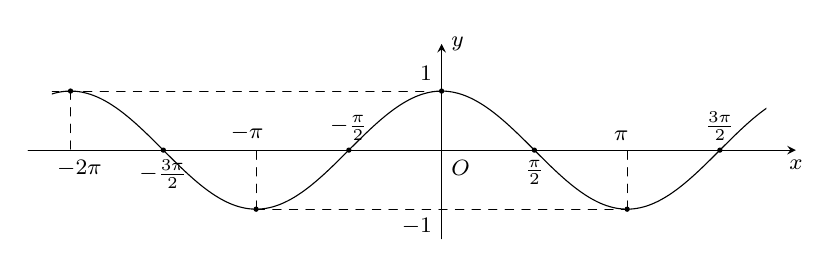
\begin{tikzpicture}[scale=0.75,>=stealth, font=\footnotesize, line join=round, line cap=round]
\def\xmin{-10} \def\xmax{10.5} \def\ymin{-1.5} \def\ymax{1.8}
\draw[->] (-7,0)--(6,0) node [below]{$x$};
\draw[->] (0,\ymin)--(0,\ymax) node [right]{$y$};
\node at (0,0) [below right]{$O$};
\clip (\xmin+3.4,\ymin+0.1) rectangle (\xmax-5,\ymax-0.1);
\draw[smooth,samples=400,domain=\xmin:\xmax] plot(\x,{cos(\x r)});
\draw[dashed] (\xmin,1)--(0,1) (-3.14,-1)--(3.14,-1);
\foreach \x in {-2*pi,-1.5*pi,-pi,-0.5*pi,0}
{\draw[fill=black] (\x,cos \x*180/pi) circle (1pt);
\draw[dashed] (\x,cos \x*180/pi)--(\x,0);
\draw[fill=black] (-\x,cos -\x*180/pi) circle (1pt);
\draw[dashed] (-\x,cos \x*180/pi)--(-\x,0);}
\node at (0,1.3) [left]{$1$};
\node at (0,-1.3) [left]{$-1$};
\node at (-2*pi+0.15,0) [below]{$-2\pi$};
\node at (-1.5*pi,0) [below]{$-\frac{3\pi}{2}$};
\node at (-pi-0.15,0) [above]{$-\pi$};
\node at (-0.5*pi,0) [above]{$-\frac{\pi}{2}$};
\node at (0.5*pi,0) [below]{$\frac{\pi}{2}$};
\node at (pi-0.1,0) [above]{$\pi$};
\node at (1.5*pi,0) [above]{$\frac{3\pi}{2}$};
\end{tikzpicture}
\end{center}
\end{enumerate} 

\loigiai{
\begin{enumerate}
\item Ta có
\begin{eqnarray*} 
&-1&\leq \cos\left[\dfrac{\pi}{4}\left( 4-\dfrac{t}{3}\right) \right]\leq 1\\ &\Leftrightarrow& - 8 \leq  8\cos\left[\dfrac{\pi}{4}\left( 4-\dfrac{t}{3}\right) \right]\leq 8\\ &\Leftrightarrow& 21 \leq 29 + 8\cos\left[\dfrac{\pi}{4}\left( 4-\dfrac{t}{3}\right) \right] \leq 37\\
&\Leftrightarrow& 21 \leq f(t)\leq 37.
\end{eqnarray*}
$\text{Max} f(t) = 37$ khi $\cos\left[\dfrac{\pi}{4}\left( 4-\dfrac{t}{3}\right) \right] = 1\Leftrightarrow \dfrac{\pi}{4}\left( 4-\dfrac{t}{3}\right) = k2\pi \Leftrightarrow t = 3(4-8k)$.\\
Do $0\leq t \leq 24$ cho nên $-\dfrac{1}{2}\leq k \leq \dfrac{1}{2}$ ta chọn $k = 0 \Rightarrow t = 12$.\\ 
Vậy nhiệt độ cao nhất trong ngày là $37$ độ C vào lúc $12$ giờ.
\item 
\begin{center}
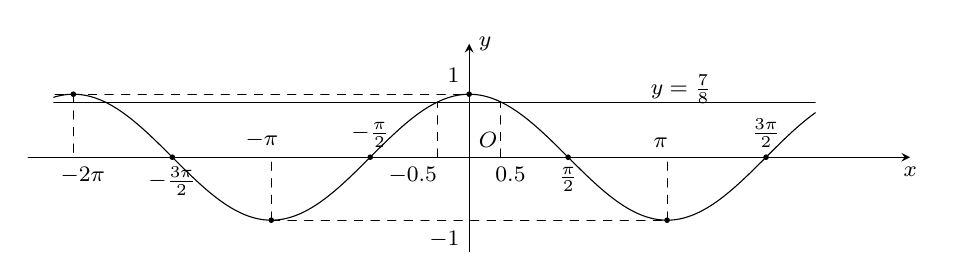
\begin{tikzpicture}[scale=0.8,>=stealth, font=\footnotesize, line join=round, line cap=round]
\def\xmin{-10} \def\xmax{10.5} \def\ymin{-1.5} \def\ymax{1.8}
\draw[->] (-7,0)--(7,0) node [below]{$x$};
\draw[->] (0,\ymin)--(0,\ymax) node [right]{$y$};
\node at (0,0) [above right]{$O$};
\clip (\xmin+3.4,\ymin+0.1) rectangle (\xmax-5,\ymax-0.1);
\draw[smooth,samples=400,domain=\xmin:\xmax] plot(\x,{cos(\x r)});
\draw[dashed] (\xmin,1)--(0,1) (-3.14,-1)--(3.14,-1);
\draw
(\xmin,7/8)--(\xmax,7/8);
\foreach \x in {-2*pi,-1.5*pi,-pi,-0.5*pi,0}
{\draw[fill=black] (\x,cos \x*180/pi) circle (1pt);
\draw[dashed] (\x,cos \x*180/pi)--(\x,0);
\draw[fill=black] (-\x,cos -\x*180/pi) circle (1pt);
\draw[dashed] (-\x,cos \x*180/pi)--(-\x,0);}
\node at (0,1.3) [left]{$1$};
\node at (0,-1.3) [left]{$-1$};
\node at (-2*pi+0.15,0) [below]{$-2\pi$};
\node at (0.161*pi+0.15,0) [below  ]{$0.5$};
\node at (-0.161*pi+0.15,0) [below left ]{$-0.5$};
\node at (4.0,0.7) [above left ]{$y = \frac{7}{8}$};
\node at (-1.5*pi,0) [below]{$-\frac{3\pi}{2}$};
\node at (-pi-0.15,0) [above]{$-\pi$};
\node at (-0.5*pi,0) [above]{$-\frac{\pi}{2}$};
\node at (0.5*pi,0) [below]{$\frac{\pi}{2}$};
\node at (pi-0.1,0) [above]{$\pi$};
\node at (1.5*pi,0) [above]{$\frac{3\pi}{2}$};
\draw[dashed] (0.5,0)--(0.5,7/8);
\draw[dashed] (-0.5,0)--(-0.5,7/8);
\end{tikzpicture}
\end{center}
Theo đề bài ta có
\begin{eqnarray*} 
&f(t)& \leq 36 \\&\Leftrightarrow& 29 + 8\cos\left[\dfrac{\pi}{4}\left( 4-\dfrac{t}{3}\right) \right] \leq 36\\ &\Leftrightarrow & \cos\left[\dfrac{\pi}{4}\left( 4-\dfrac{t}{3}\right) \right] \leq \dfrac{7}{8}\\& \Leftrightarrow& -0{,}5  \leq \dfrac{\pi}{4}\left( 4-\dfrac{t}{3}\right) \leq 0{,}5\\& \Leftrightarrow& 10{,}1 \leq t \leq 13{,}9.
\end{eqnarray*}
\end{enumerate}

Như vậy để tránh nhiệt độ trên $36^\circ$C thì các công nhân làm việc từ $10{,1}$ giờ đến $13{,}9$ giờ.
}
\end{ex}

\begin{ex}[THPT Chuyên Quốc Học Huế 24-25]%[1D1V5-6]%[Dự án đề kiểm tra Toán 11 HKI NH24-25- Nguyễn Ngọc Dũng]
	\immini{
		Một chiếc đu quay có tâm của vòng quay ở độ cao $35$ m so với mặt đất, khoảng cách từ tâm vòng quay đến vị trí gắn các cabin là $30$ m. Thời gian thực hiện mỗi vòng của đu quay là 3 phút 20 giây. Một hành khách vào cabin số 1 được gắn tại vị trí $A$ thấp nhất của vòng quay (tham khảo hình vẽ), sau $t$ giây kể từ lúc quay, vị trí $A$ cách mặt đất $h(t)$ mét. Biết rằng $h(t)$ có dạng $h(t)=a \cos (\omega t)+b(a, b, \omega$ là hằng số). Xác định $a, b, \omega$ và tính thời gian ngắn nhất kể từ lúc quay để vị trí $A$ cách mặt đất $25$ m (thời gian làm tròn đến hàng đơn vị).
	}{
		\begin{tikzpicture}[scale=0.5,font=\small,line join=round,line cap=round,>=stealth]
			\tikzset{declare function={g=0;}}
			\coordinate (O) at (0,0);
			\coordinate (A) at (0:4.4);
			\coordinate (M) at (30+g:4.4);
			\pgfmathsetmacro{\gx}{60-g};
			\coordinate (v) at ($(M)+(120+g:3.3)$);
			\coordinate (vx) at ($(M)+(180:3.3*cos \gx)$);
			\draw[thick] (O) circle(4.4) (O) circle(3.53);
			\foreach \t in {0,1,...,11}{
				\draw[very thick,fill] (O)--(g+30*\t:4.4)circle(0.06);
				\begin{scope}[shift={(g+30*\t:4.4)}]
					\draw[fill=teal] (-0.27,0)--(0.27,0)--(0.36,-0.18)--(-0.36,-0.18)--cycle
					(0.32,-0.18)--(0.32,-0.54) (-0.32,-0.18)--(-0.32,-0.54)
					(-0.4,-0.54)--(0.4,-0.54)--(0.27,-1)--(-0.27,-1)--cycle;
			\end{scope}}
			\draw[fill=gray!70!yellow] (0.2,0)--(2.35,-5.53)--(3.65,-5.53)--(3.65,-6.02)--(1.95,-6.02)--(0,-0.85)--(-1.95,-6.02)--(-3.65,-6.02)--(-3.65,-5.53)--(-2.35,-5.53)--(-0.2,0)--cycle;
			\draw[fill=gray!10!yellow] (O) circle(0.34);
			\draw[fill] (-5,-5.85)--(0,-5.85) node[below]{$A$} circle(0.08)--(6.4,-5.85);
		\end{tikzpicture}
	}
	\loigiai{
		Ta có $3$ phút $20$ giây bằng $200$ giây. \\
		Chu kì của vòng quay là 
		$\dfrac{2\pi}{\omega} = 200 \Leftrightarrow \omega = \dfrac{\pi}{100}.$\\
		Suy ra $h(t)=a \cos \left(\dfrac{\pi}{100} t\right)+b$ \\
		$h(t)$ có giá trị nhỏ nhất và lớn nhất lần lượt là $5$ và $65$. Do đó \\
		Với $t=0$ ta có $h(0)=5 \Leftrightarrow a + b =5$. \\
		Với $t=100$ ta có $h(100)=65 \Leftrightarrow -a + b =65$. \\
		Ta có  $\heva{&a+b=5 \\& -a+b=65} \Leftrightarrow \heva{&a=-30 \\& b=35.}$ \\
		Suy ra $h(t) = -30\cos \left(\dfrac{\pi}{100} t \right) +35$. \\
		Để cabin A cách mặt đất 25 mét thì 
		\allowdisplaybreaks 
		\begin{eqnarray*}
			&& h(t)=25\\
			&\Leftrightarrow& -30\cos \left(\dfrac{\pi}{100} t \right) +35=25 \\
			&\Leftrightarrow & \cos \left(\dfrac{\pi}{100} t \right) = \dfrac{1}{3}
		\end{eqnarray*}
		Gọi $\alpha \in [0;\pi]$ là góc thoả mãn $\cos \alpha = \dfrac{1}{3}$. Khi đó 
		$$\cos \left(\dfrac{\pi}{100} t \right) = \cos \alpha \Leftrightarrow \hoac{&t=\dfrac{100}{\pi}  \alpha +200k\\&t=-\dfrac{100}{\pi} \alpha+200k}, (k\in\mathbb{Z}).$$
		Với $t=\dfrac{100}{\pi} \alpha+200k \ge 0 \Leftrightarrow k \ge -0,196 $. \\
		Giá trị dương nhỏ nhất của $t$  là  $t= \dfrac{100}{\pi} \alpha+200\cdot0 \approx 39$. \\
		Với $t=-\dfrac{100}{\pi} \alpha+200k \ge 0 \Leftrightarrow k \ge 0,196$. \\
		Giá trị dương nhỏ nhất của $t$  là  $t = -\dfrac{100}{\pi} \alpha+200 \cdot 1 \approx 161$. \\
		Do đó thời gian ngắn nhất từ lúc bắt đầu đến khi cabin A cách mặt đất 25 mét là 39 giây. 
	}
\end{ex}
